\section{Signal variable studies for T2tt like signatures}
\label{sec:sigvarstudy}

This appendix discusses investigations on various variables suitable for signal discriminating variables. As signal we have four mass points of top squark pair production where both top squark decays are $\PSQt\to\cPqt\PSGczDo$.

The distributions on those variables are investigated, and relative sensitivity values are given for ad-hoc chosen selection criteria.
Although not chosen, some of these variables might still be useful in a later iteration of this analysis when either more data will be available or these variables are less correlated to current signal variable and such could be chosen by a multivariate classifier.

This study has been performed before the final event selection had been decided. Therefore, the yields will not match those of the analysis described above. However, the relative yields for the signal regions defined in this section should be largely unaffected by the differences in the event selection.

Another difference for this section is that the simulation had been normalized to 5 or 10\fbinv.

\subsection{Event selection for this study, signal mass points}
\label{sec:sigvarstudy:evtselection}

\begin{itemize}
\item First vertex is good.
\item Exactly one selection lepton:
	\begin{itemize}
	\item Electrons: $\pt>40\GeV$, $|\eta|<2.1$, medium ID, miniiso$ < 0.1$,
	\item Muons: $\pt>30\GeV$, $|\eta|<2.1$, medium ID, miniiso$ < 0.2$,
	\end{itemize}
\item No additional veto lepton:
	\begin{itemize}
	\item Electrons: $\pt>10\GeV$, $|\eta|<2.4$, veto ID, miniiso$ < 0.2$,
	\item Muons: $\pt>10\GeV$, $|\eta|<2.4$, loose ID, miniiso$ < 0.2$,
	\end{itemize}
\item  At least four jets ($\pt>30\GeV$, $|\eta|<2.4$, loose ID),
\item  At least on b-jet (medium CSVv2+IVF WP),
\item  $\MET>200\GeV$ (type-1 corrected),
\item  $\MT>150\GeV$,
\item  $\minDPhiMETjet>0.8$.
\end{itemize}
In addition, four selection stages were investigated:
\begin{enumerate}
\item Preselection as above,
\item Preselection plus $\MET>300\GeV$,
\item Preselection plus $\MET>300\GeV$, $\chi^2_{\mathrm{had.}\cPqt}<10$,
\item Preselection plus $\MET>300\GeV$, $\chi^2_{\mathrm{had.}\cPqt}<10$, $\MTtW>200\GeV$.
\end{enumerate}
The $\chi^2_\mathrm{had.top}$ variable was calculated similar to the 8\TeV analysis~\cite{Chatrchyan:2013xna}, however with a flat jet energy resolution of 10\%.

For this study, PHYS14 simulation was used. The signal mass points are:
\begin{itemize}
\item $M_{\PSQt} = 425\GeV$, $M_{\PSGczDo} = 325\GeV$,
\item $M_{\PSQt} = 500\GeV$, $M_{\PSGczDo} = 325\GeV$,
\item $M_{\PSQt} = 650\GeV$, $M_{\PSGczDo} = 325\GeV$,
\item $M_{\PSQt} = 850\GeV$, $M_{\PSGczDo} = 100\GeV$.
\end{itemize}

\subsection{Signal variables under study}
\label{sec:sigvarstudy:variables}

\subsubsection{\MTtW}

The \MTtW variable~\cite{Bai:2012gs} is defined as
\begin{align}
\MTt^W = &\min\left\{m_y\text{ consistent with } \left[ p_1^2 = 0, \right.\right. 
(p_1+p_\ell)^2 = p_2^2 = M_{\PW}, \\
& \ptvec^1+\ptvec^2 = \VEtmiss, 
\left.\left. (p_1+p_\ell+p_{\cPqb_1})^2=(p_2+p_{\cPqb_2})^2 = m_y^2,\right]\right\} \nonumber
\end{align}
The basic idea is to try to split \MET into its components due to the lost \PW boson and $\cPgn_1$, such that you get two symmetric masses consistent with event kinematics of a lost lepton in $\cPqt\cPaqt$.
The output is the fitted mass $m_y$.
Therefore, the variable is specifically designed to reduce dileptonic $\cPqt\cPaqt$ with a lost lepton for a single-lepton top squark search, for which $m_y \approx M_{\cPqt}$.

For further details, please see also section {\color{red} REFERENCE SECTION ABOVE}.

Figure~\ref{fig:sigvarstudy:MT2WTopness:MT2W} shows the \MTtW distribution after preselection plus $\MET>300\GeV$. As a test selection $\MTtW>200\GeV$ was chosen.

\begin{figure}
\subfigure[\MTtW distribution.]{
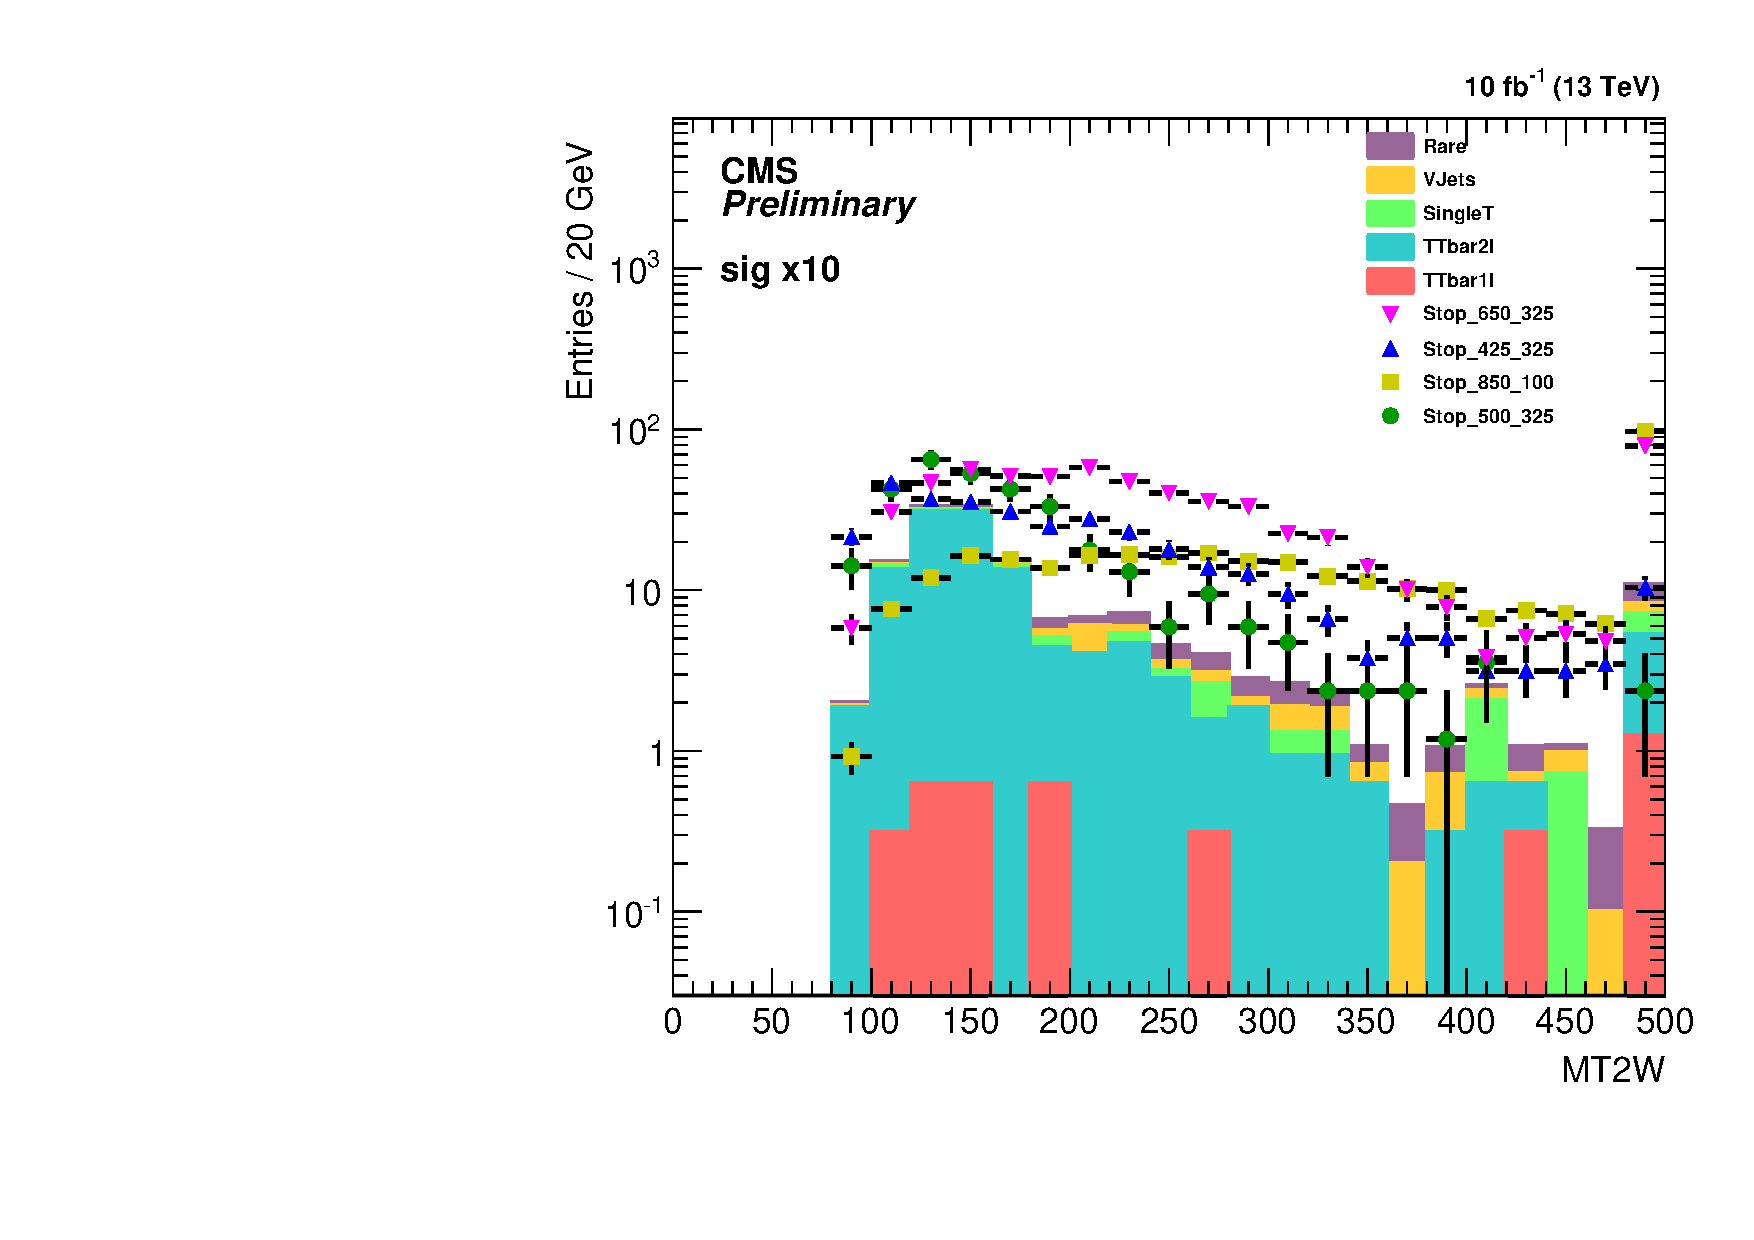
\includegraphics[width=0.49\textwidth]{Figures/SignalVariableStudies/MT2W.pdf}
\label{fig:sigvarstudy:MT2WTopness:MT2W}
}
\subfigure[Topness distribution.]{
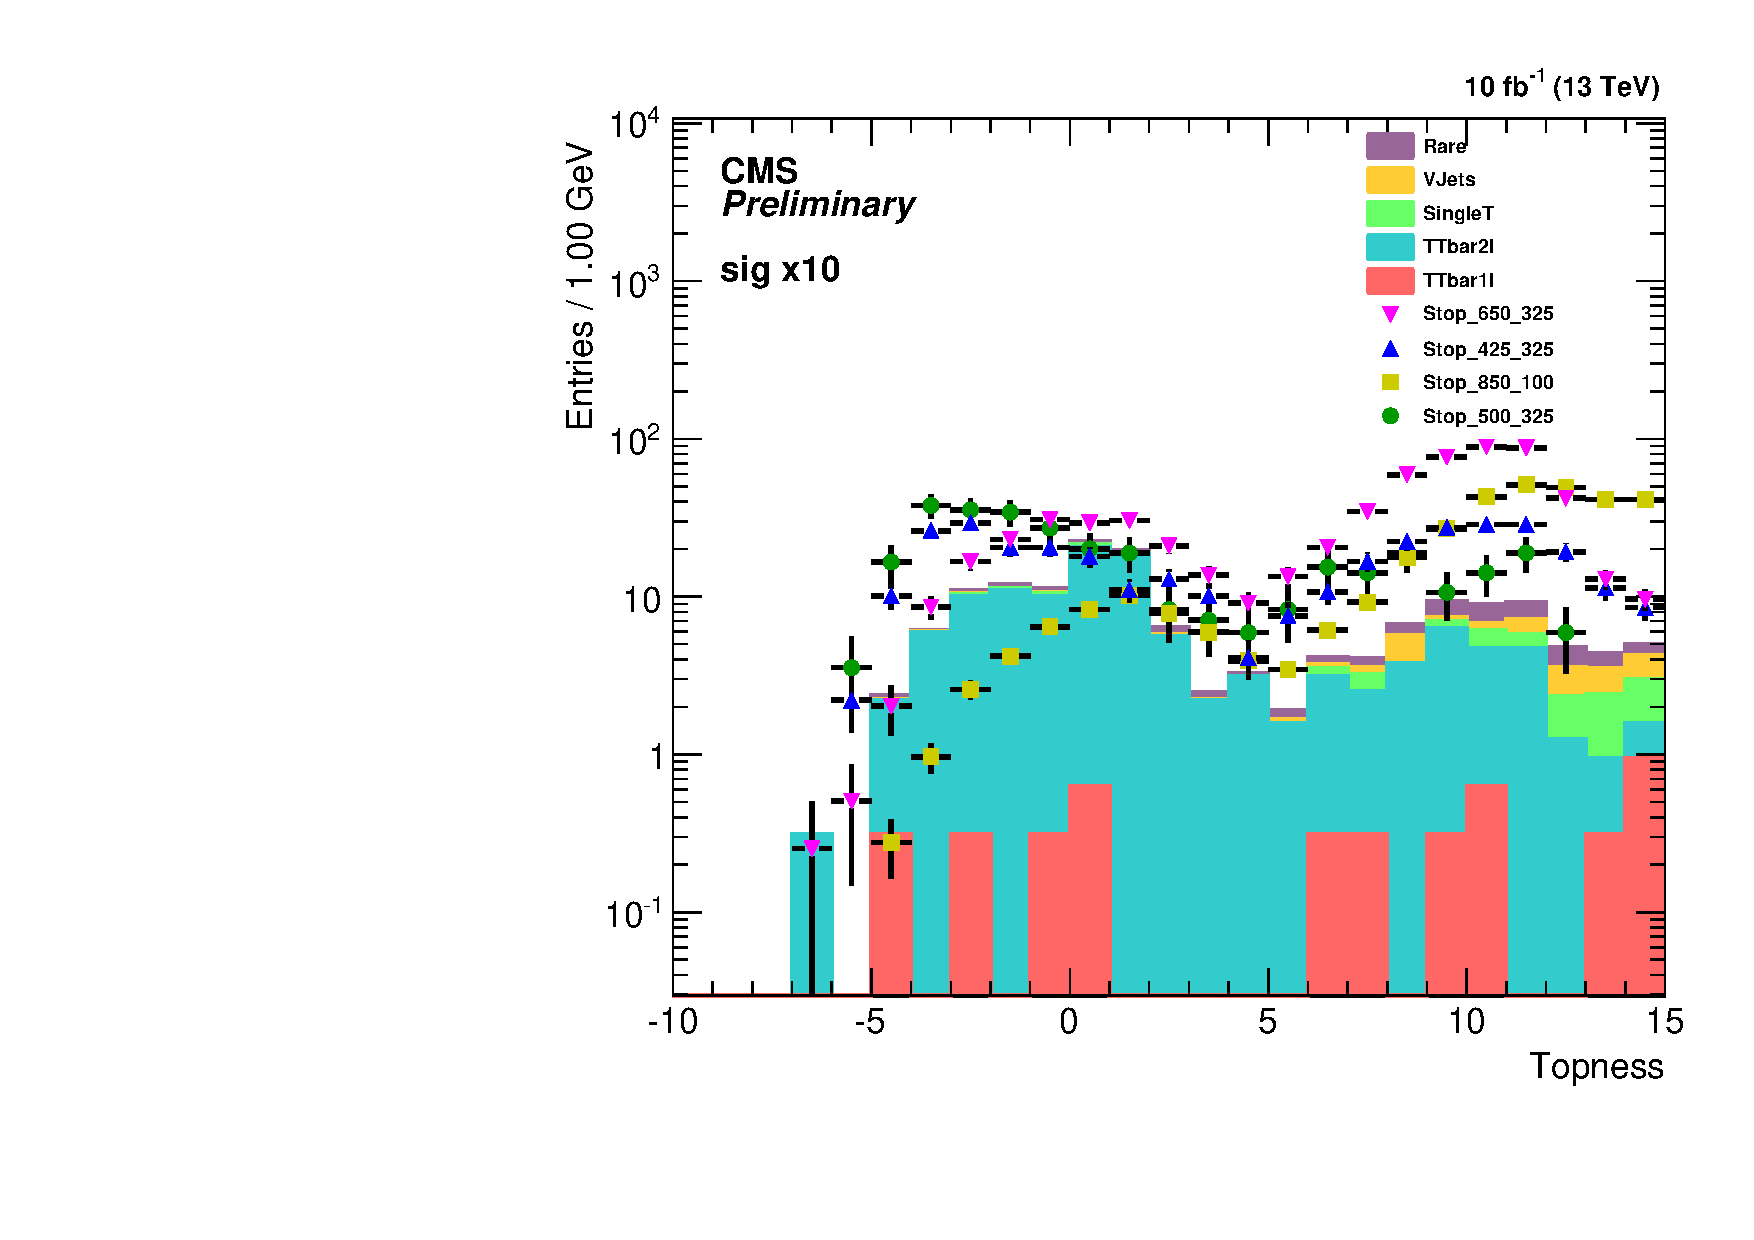
\includegraphics[width=0.49\textwidth]{Figures/SignalVariableStudies/Topness.pdf}
\label{fig:sigvarstudy:MT2WTopness:Topness}
}
\caption{\label{fig:sigvarstudy:MT2WTopness} The \MTtW (left) and topness (right) distributions.}
\end{figure}

\subsubsection{Topness}
\label{sec:sigvarstudy:topness}

The topness variable~\cite{Graesser:2012qy} is defined as
\begin{align} t = &\ln(\min S)~\text{ with }~ S(\vec{p}_\PW, p_{\cPgn,z}) = \\
 &\frac{(M_\PW^2-(p_\cPgn+p_\ell)^2)^2}{a_\PW^4} + \frac{(M_\cPqt^2-(p_{\cPqb_1}+p_\ell+p_\cPgn)^2)^2}{a_\cPqt^4}
 + \frac{(M_\cPqt^2 - (p_{\cPqb_2}+p_\PW)^2)^2}{a_t^4} + \frac{(4M_\cPqt^2-(\sum p_i)^2)^2}{a_\mathrm{CM}^4}. \nonumber
 \end{align}
Here, the $a$ terms are resolution terms with values $a_\PW = 5\GeV$, $a_\cPqt = 15\GeV$, $a_\mathrm{CM} = 1\TeV$.
Thus, the topness variable uses a similar idea as for \MTtW, but including the top quark mass requirement, and resolution terms $a$.

The selection of two b jets is done the same as for the \MTtW variable.

Figure~\ref{fig:sigvarstudy:MT2WTopness:Topness} shows the topness distribution after preselection plus $\MET>300\GeV$. As a test selection $t>9$ was chosen.


\subsubsection{Modified topness}
\label{sec:sigvarstudy:modtopness}

After studying the topness variable in great detail, it was found that two terms diminish the signal discriminator power at high values of the topness variable. Therefore a modification was introduced:
\begin{equation}
t_\mathrm{mod} = \ln(\min S)~\text{ with }~ S(\vec{p}_\PW, p_{\cPgn,z}) = \frac{(M_\PW^2-(p_\cPgn+p_\ell)^2)^2}{a_\PW^4} + \frac{(M_\cPqt^2 - (p_{\cPqb_2}+p_\PW)^2)^2}{a_\cPqt^4}.
\end{equation}
The top quark mass constraint for the top quark decay with the reconstructed lepton was dropped, as well as the center-of-mass constraint.

The reason is the following: The W boson mass constraint for the top quark decay with the reconstructed lepton already constraints the \MET splitting well enough. This can get diminished if the jet used in the corresponding top quark mass constraint does not come from the top quark decay (like mistagged jet or b-jet from gluon splitting). Dropping the center-of mass term has only a small effect.

Figure~\ref{fig:sigvarstudy:TopnessModMT2lbb:TopnessMod} shows the modified topness distribution after preselection plus $\MET>300\GeV$. As a test selection $t_\mathrm{mod}>7$ was chosen.

\begin{figure}
\subfigure[Modified topness distribution.]{
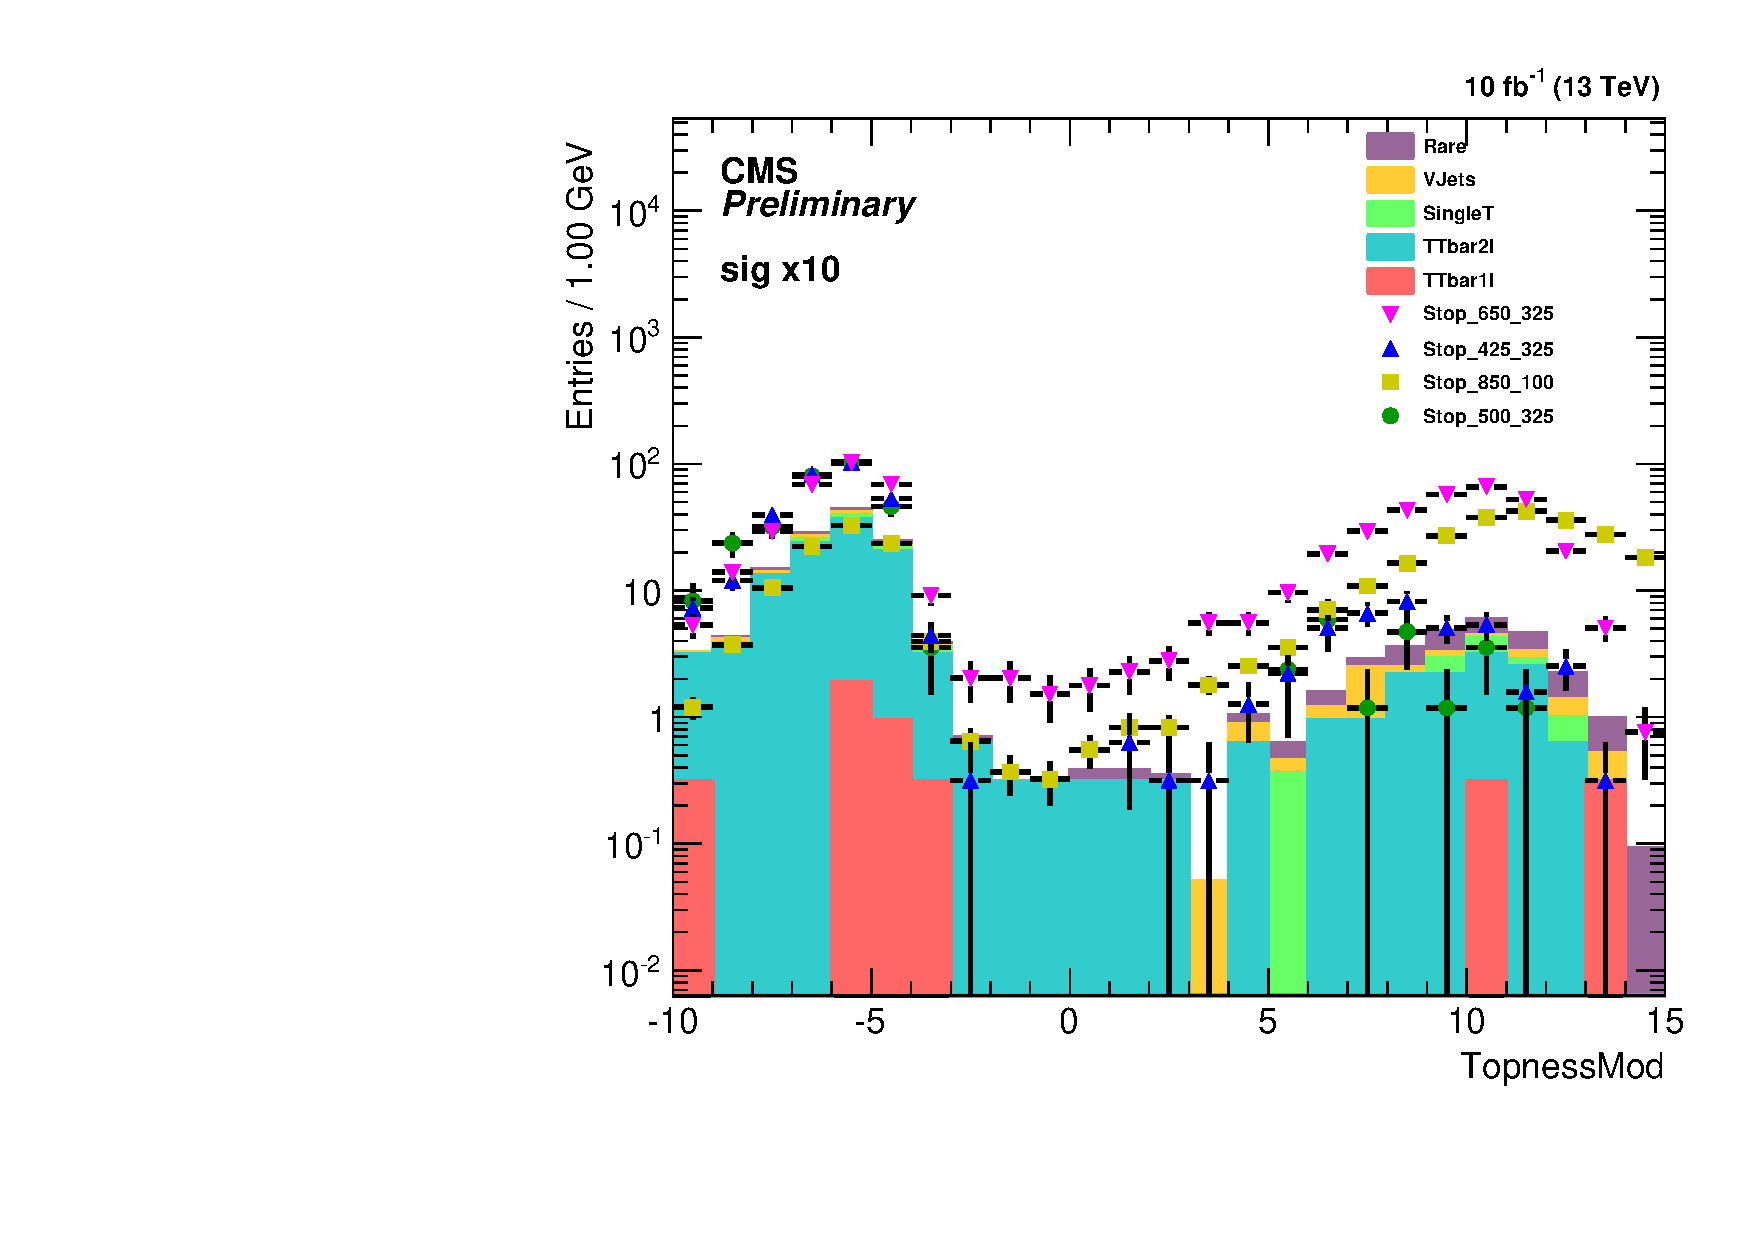
\includegraphics[width=0.49\textwidth]{Figures/SignalVariableStudies/TopnessMod.pdf}
\label{fig:sigvarstudy:TopnessModMT2lbb:TopnessMod}
}
\subfigure[$\MTt(\ell\cPqb,\cPqb)$ distribution.]{
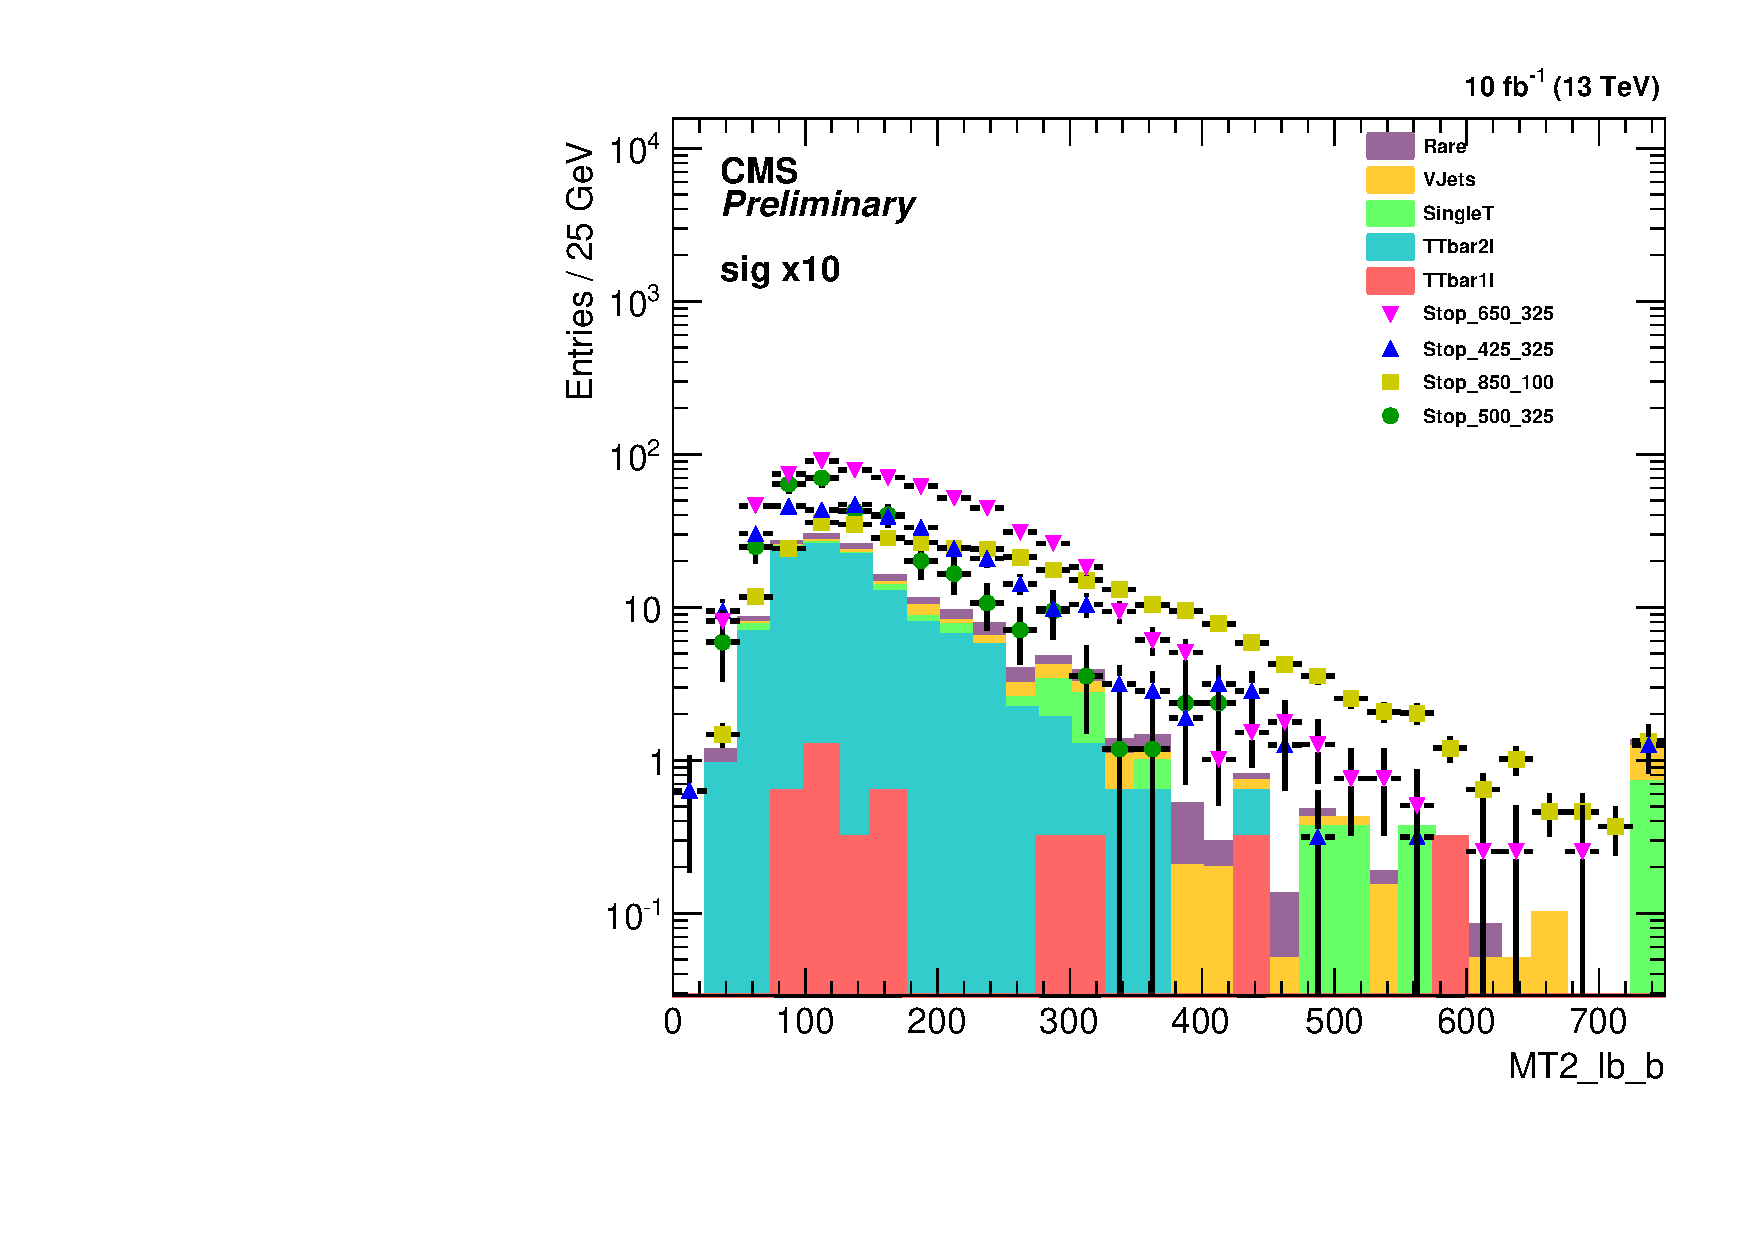
\includegraphics[width=0.49\textwidth]{Figures/SignalVariableStudies/MT2_lb_b.pdf}
\label{fig:sigvarstudy:TopnessModMT2lbb:MT2lbb}
}
\caption{\label{fig:sigvarstudy:TopnessModMT2lbb} The modified topness (left) and $\MTt(\ell\cPqb,\cPqb)$ (right) distributions.}
\end{figure}

\subsubsection{$\MTt(\ell\cPqb,\cPqb)$}

The \MTt variable~\cite{Lester:1999tx} is defined as 
\begin{equation}
 \MTt(M_{\tilde{\chi}}) = \min_{\scriptscriptstyle\ptvec^{\tilde{\chi}(1)} + \ptvec^{\tilde{\chi}(2)} = \VEtmiss} \left[ \max \left( \MT^{(1)} , \MT^{(2)} \right) \right].
\end{equation}
This variable was designed to measure mass of pair-produced particles, each decaying semi-invisible. As visible objects, we take here ($1\ell + 1\cPqb$) and ($1\cPqb$), and the testmass $M_{\tilde{\chi}} = 0$.
The selection of two b jets is done the same as for the \MTtW variable.

Figure~\ref{fig:sigvarstudy:TopnessModMT2lbb:MT2lbb} shows the $\MTt(\ell\cPqb,\cPqb)$ distribution after preselection plus $\MET>300\GeV$. As a test selection $\MTt(\ell\cPqb,\cPqb)>175\GeV$ was chosen.

\subsubsection{(Massless) $\MTt(\ell\cPqb,\cPqb\cPq\cPq)$}

We can also define the \MTt variable with two visible systems as ($1\ell + 1\cPqb$) and ($1\cPqb+2\cPq$). The assumption is to fully reconstruct the top squark pair production signature. While the choice of b jets is kept the same as in the previous sections, for the ``normal'' jets, we loop over all jet pair combinations, that do not include the selected b jets, and choose that combination that yields smallest $\MTt(\ell\cPqb,\cPqb\cPq\cPq)$.

When studying its distribution (see figure~\ref{fig:sigvarstudy:MT2lbbqq:massive}), we find no discrimination power. As found in an earlier search using the \MTt variable~\cite{Khachatryan:2015vra}, the mass term of the visible systems are the reason for this effect. As done in this search, after removing the visible object mass in the \MTt calculation, seen in figure~\ref{fig:sigvarstudy:MT2lbbqq:massless}, the signal discrimination is restored. However, the signal efficiency is also strongly reduced. For this (massless) variable, a test selection of $\MTt(\ell\cPqb,\cPqb\cPq\cPq)>175\GeV$ was chosen.


\begin{figure}
\subfigure[Massive $\MTt(\ell\cPqb,\cPqb\cPq\cPq)$ distribution.]{
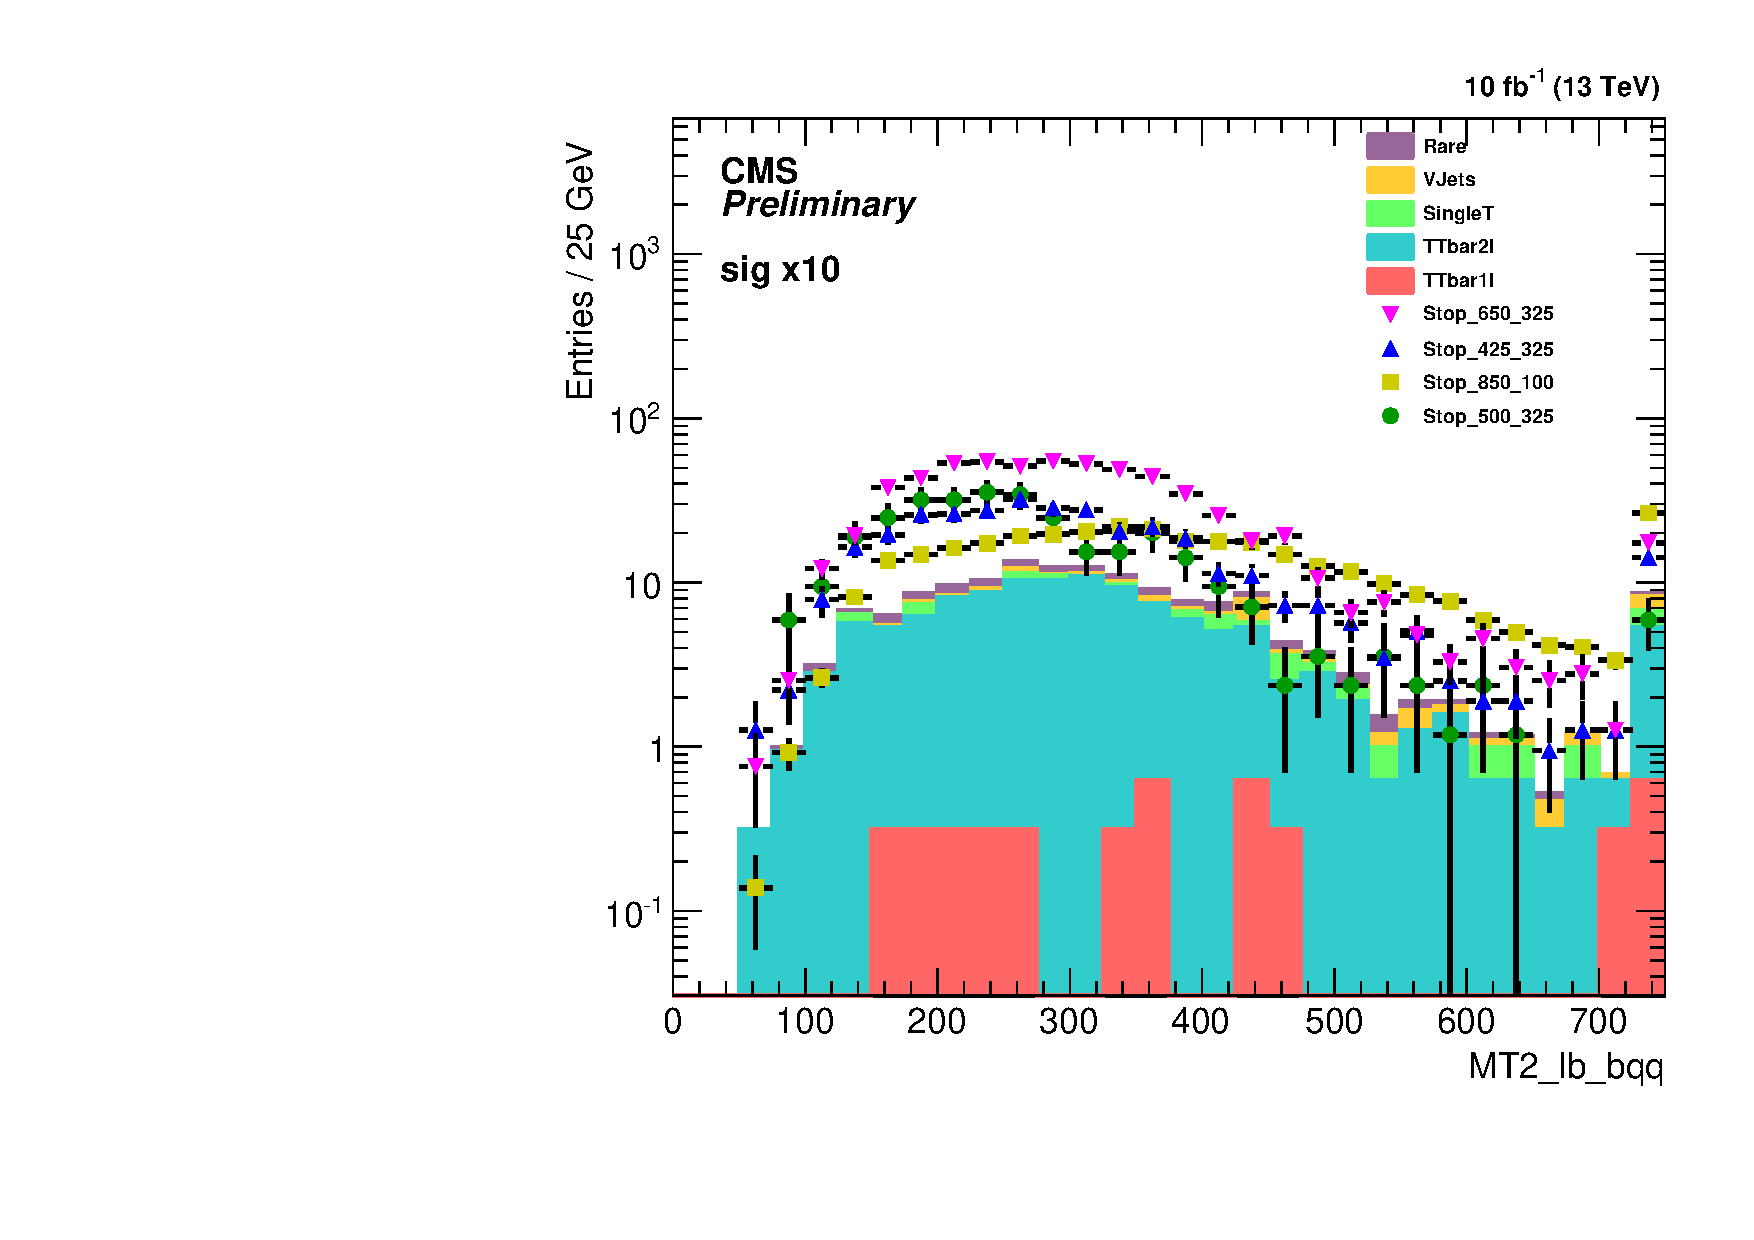
\includegraphics[width=0.49\textwidth]{Figures/SignalVariableStudies/MT2_lb_bqq.pdf}
\label{fig:sigvarstudy:MT2lbbqq:massive}
}
\subfigure[Massless $\MTt(\ell\cPqb,\cPqb\cPq\cPq)$ distribution.]{
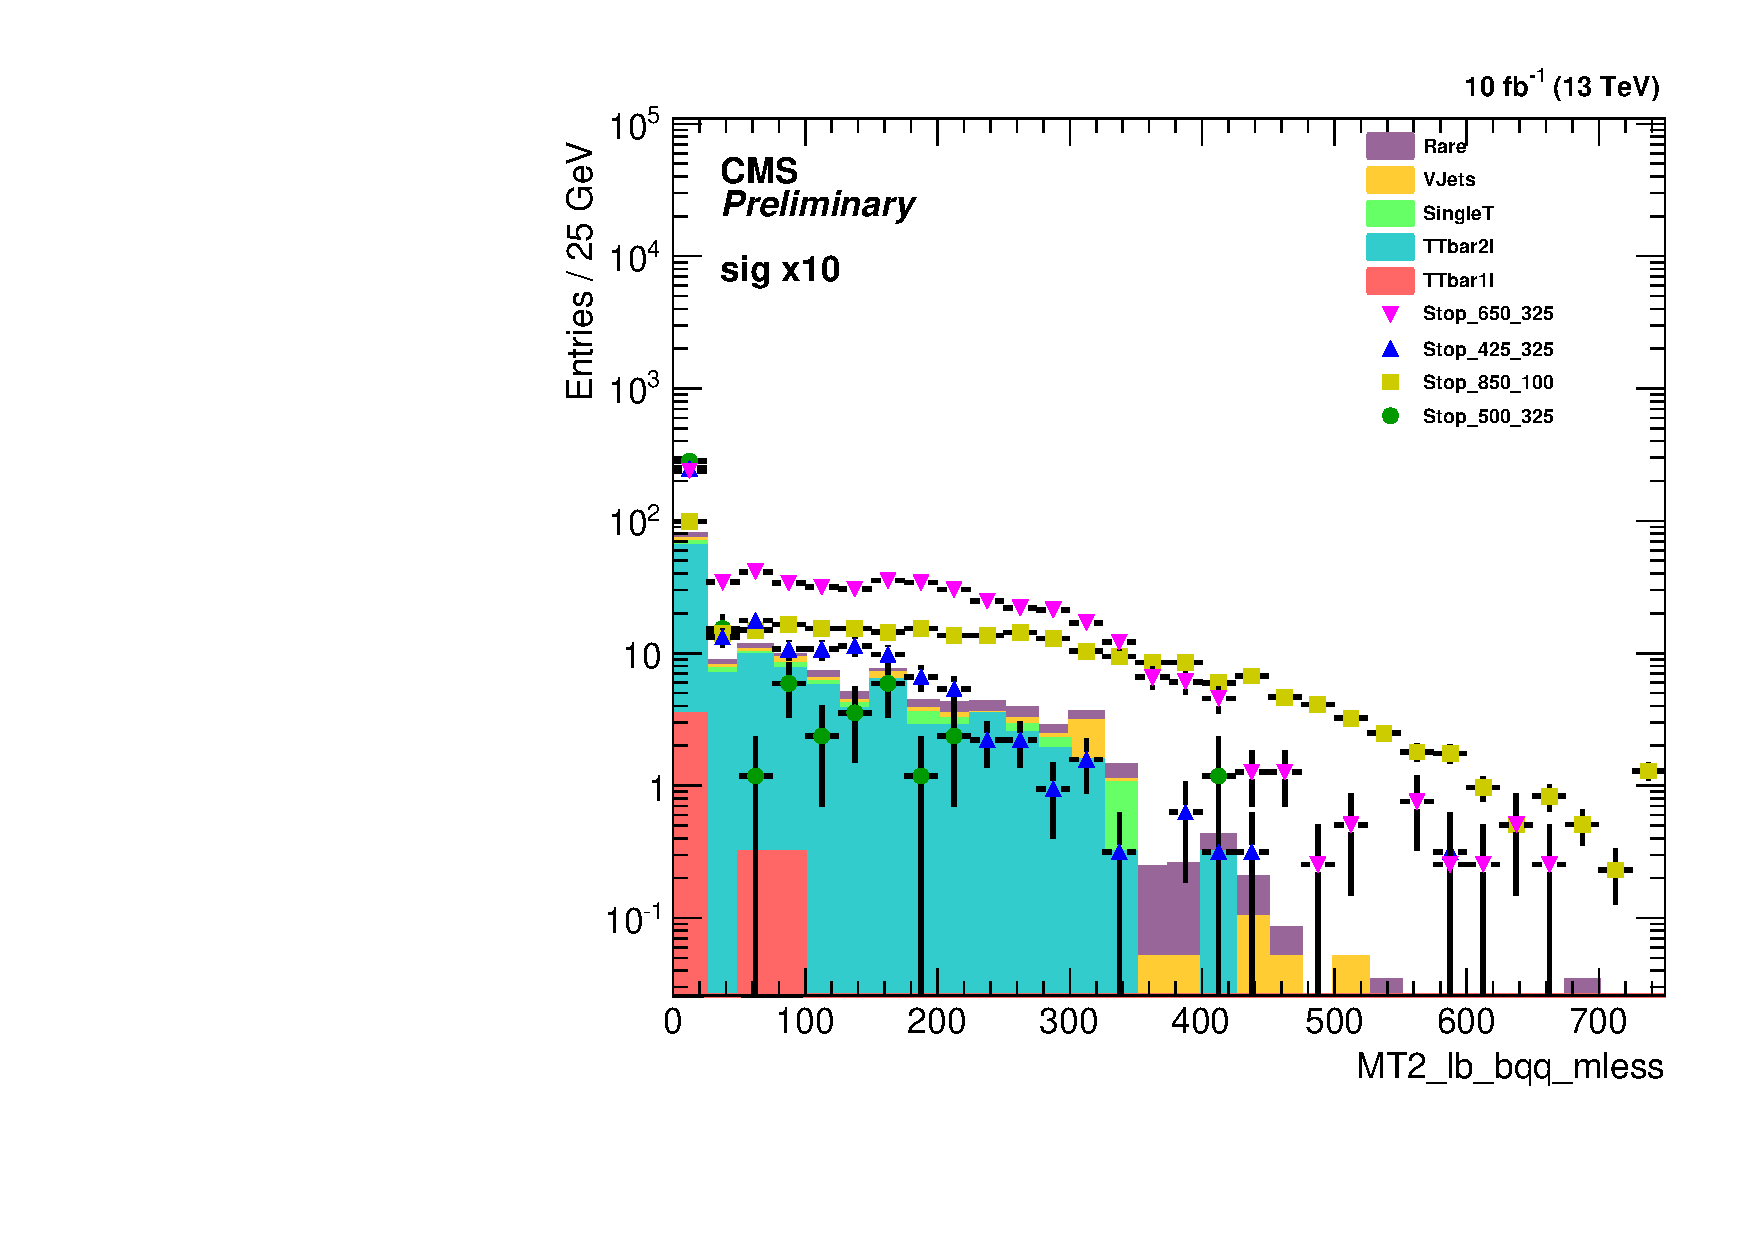
\includegraphics[width=0.49\textwidth]{Figures/SignalVariableStudies/MT2_lb_bqq_mless.pdf}
\label{fig:sigvarstudy:MT2lbbqq:massless}
}
\caption{\label{fig:sigvarstudy:MT2lbbqq} Massive (left) and massless (right) $\MTt(\ell\cPqb,\cPqb\cPq\cPq)$ distributions.}
\end{figure}

\subsubsection{(Massless) $\MTt(\ell,\cPq\cPq)$}

As it can be guessed, this variable is similar as in the section before, but without the requirements of the two b-jets. Such a variable could be sensitive for the production of charginos as in $\PSQt\to\cPqb\PSGcpmDo$, $\PSGcpmDo\to\PW\PSGczDo$.

Figure~\ref{fig:sigvarstudy:MT2lqq} shows the (massless) $\MTt(\ell,\cPq\cPq)$ distribution after preselection plus $\MET>300\GeV$. As a test selection $\MTt(\ell,\cPq\cPq)>50(60)\GeV$ was chosen.

\begin{figure}
\subfigure[Massive $\MTt(\ell,\cPq\cPq)$ distribution.]{
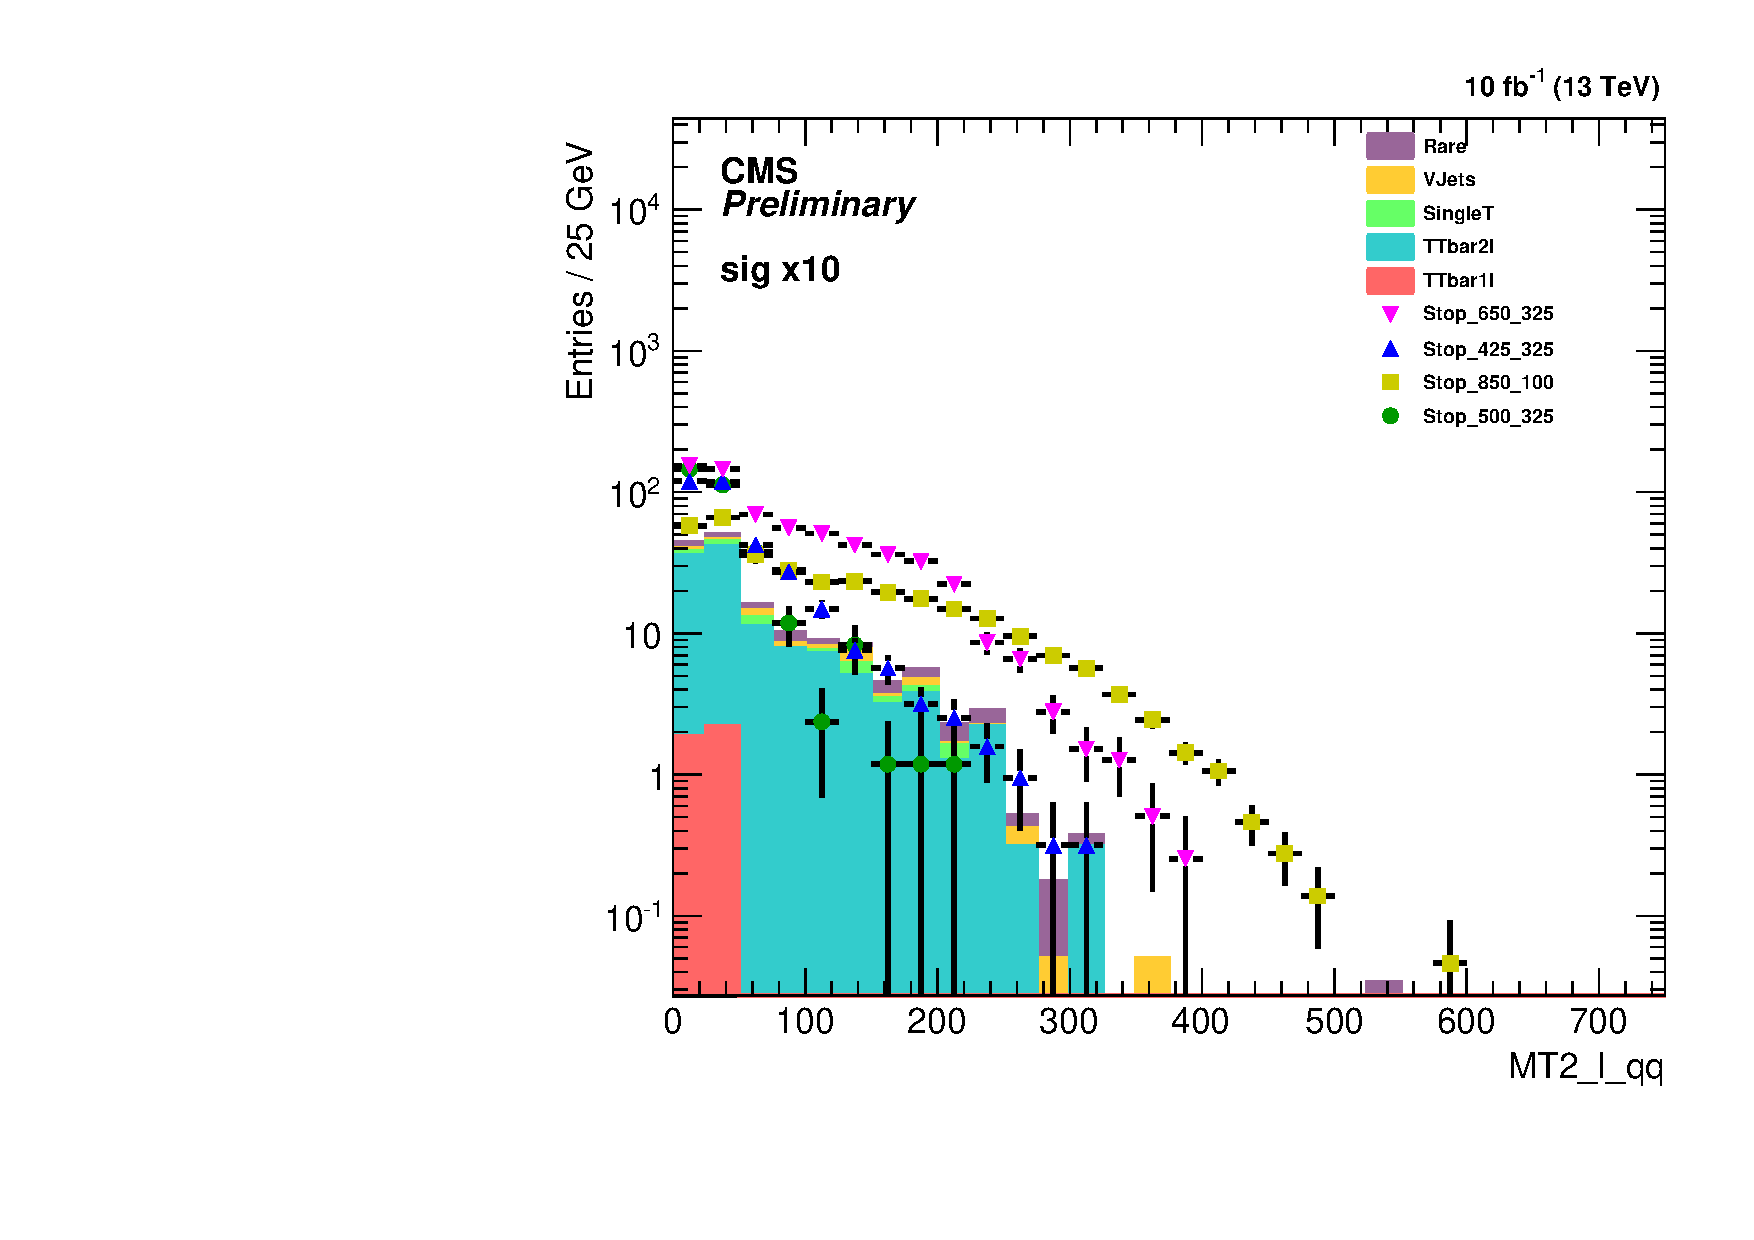
\includegraphics[width=0.49\textwidth]{Figures/SignalVariableStudies/MT2_l_qq.pdf}
\label{fig:sigvarstudy:MT2lqq:massive}
}
\subfigure[Massless $\MTt(\ell\cPqb,\cPqb\cPq\cPq)$ distribution.]{
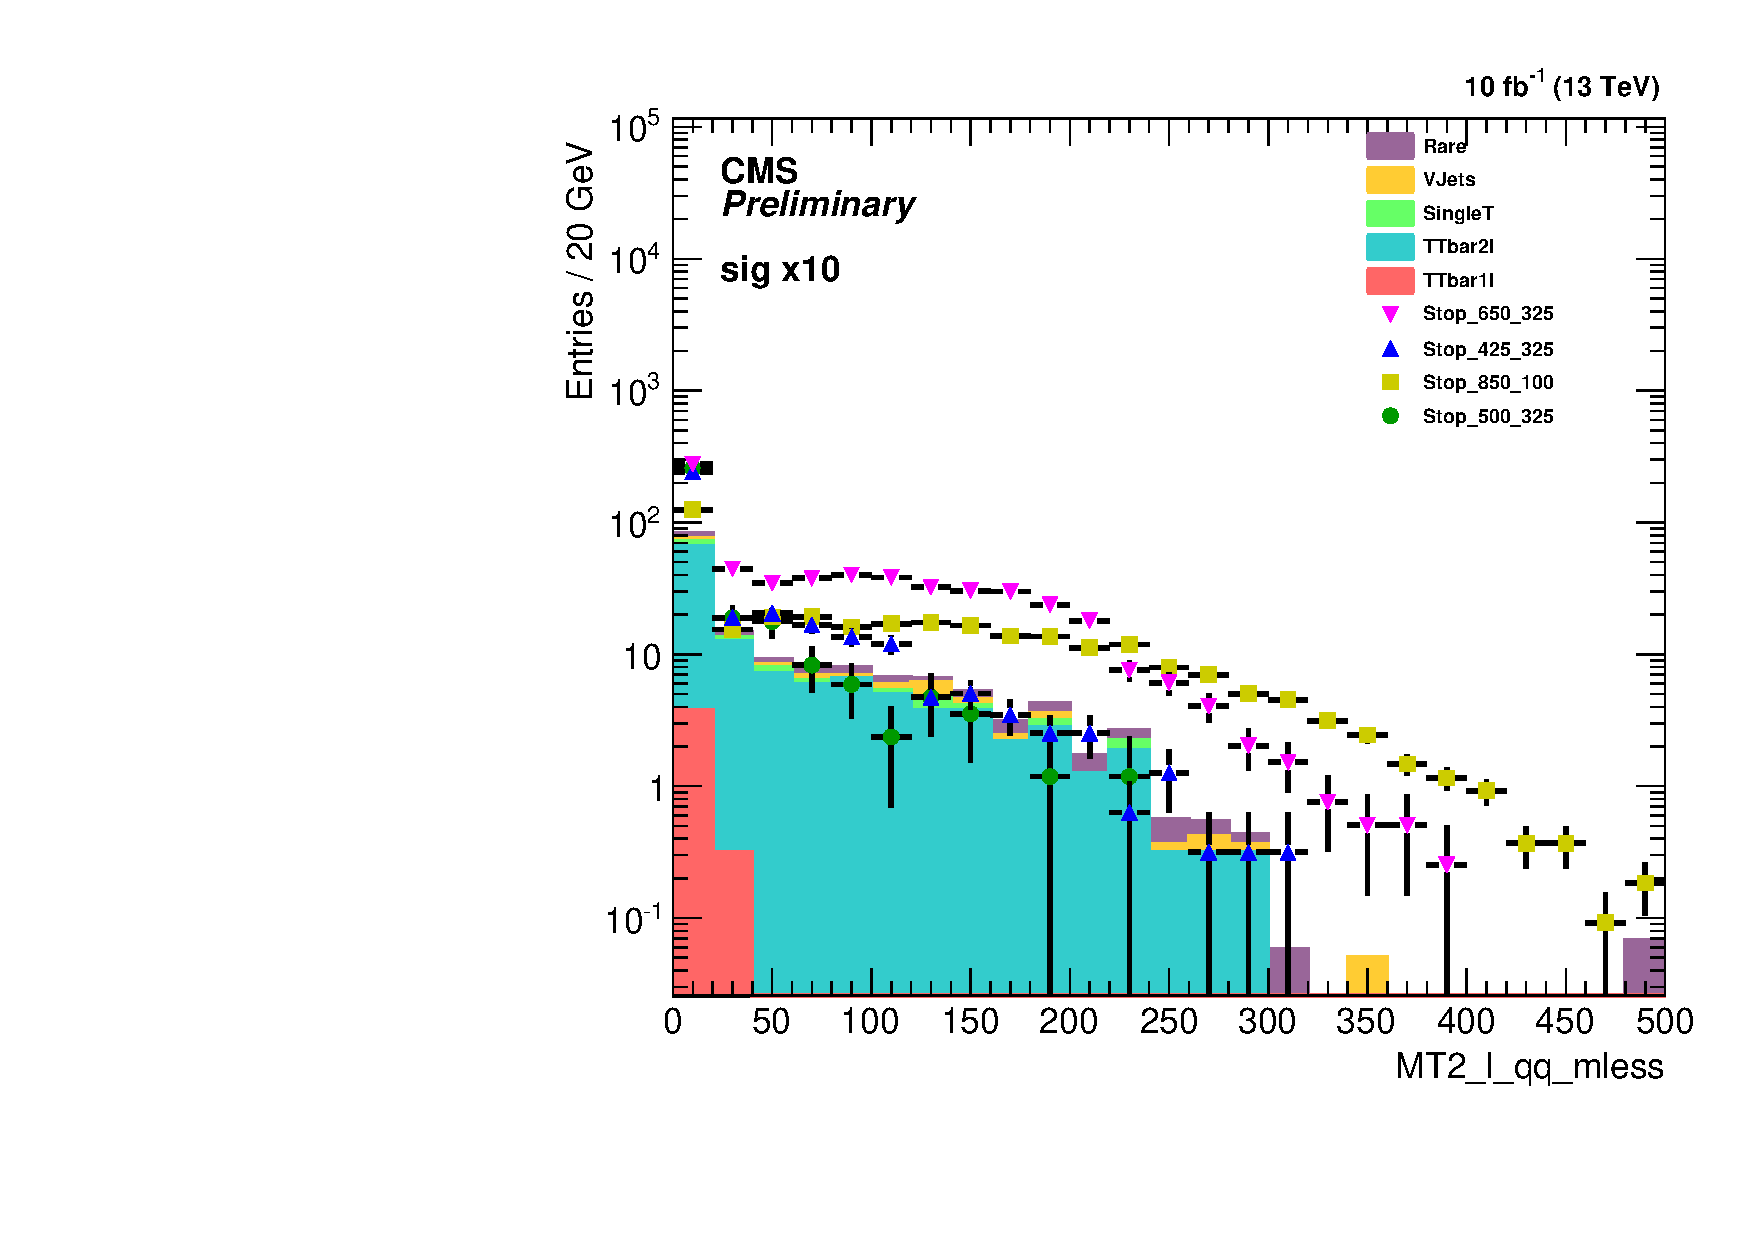
\includegraphics[width=0.49\textwidth]{Figures/SignalVariableStudies/MT2_l_qq_mless.pdf}
\label{fig:sigvarstudy:MT2lqq:massless}
}
\caption{\label{fig:sigvarstudy:MT2lqq} Massive (left) and massless (right) $\MTt(\ell,\cPq\cPq)$ distributions.}
\end{figure}

\subsubsection{$R_M$}
The $R_M$ variable~\cite{An:2015uwa} targets the compressed spectra signatures (small $\Delta M$ between the top squark and the LSP masses).
The variable is defined as 
\begin{equation}
R_M =  \frac{\MET}{\pt(j_1)} \approx \frac{\MET}{\pt(j_\mathrm{ISR})}.
\end{equation}
The idea is that the event is tagged via an ISR jet. Thus, for signal We expect a balance of \MET and the leading jet, while for SM background, lower values of $R_M$ are also possible.
For the leading jet, we require $\pt>300\GeV$.

Figure~\ref{fig:sigvarstudy:RMMTq:RM} shows the $R_M$ distribution after preselection plus $\MET>300\GeV$. As a test selection $R_M>0.8$ was chosen.

\begin{figure}
\subfigure[$R_M$ distribution.]{
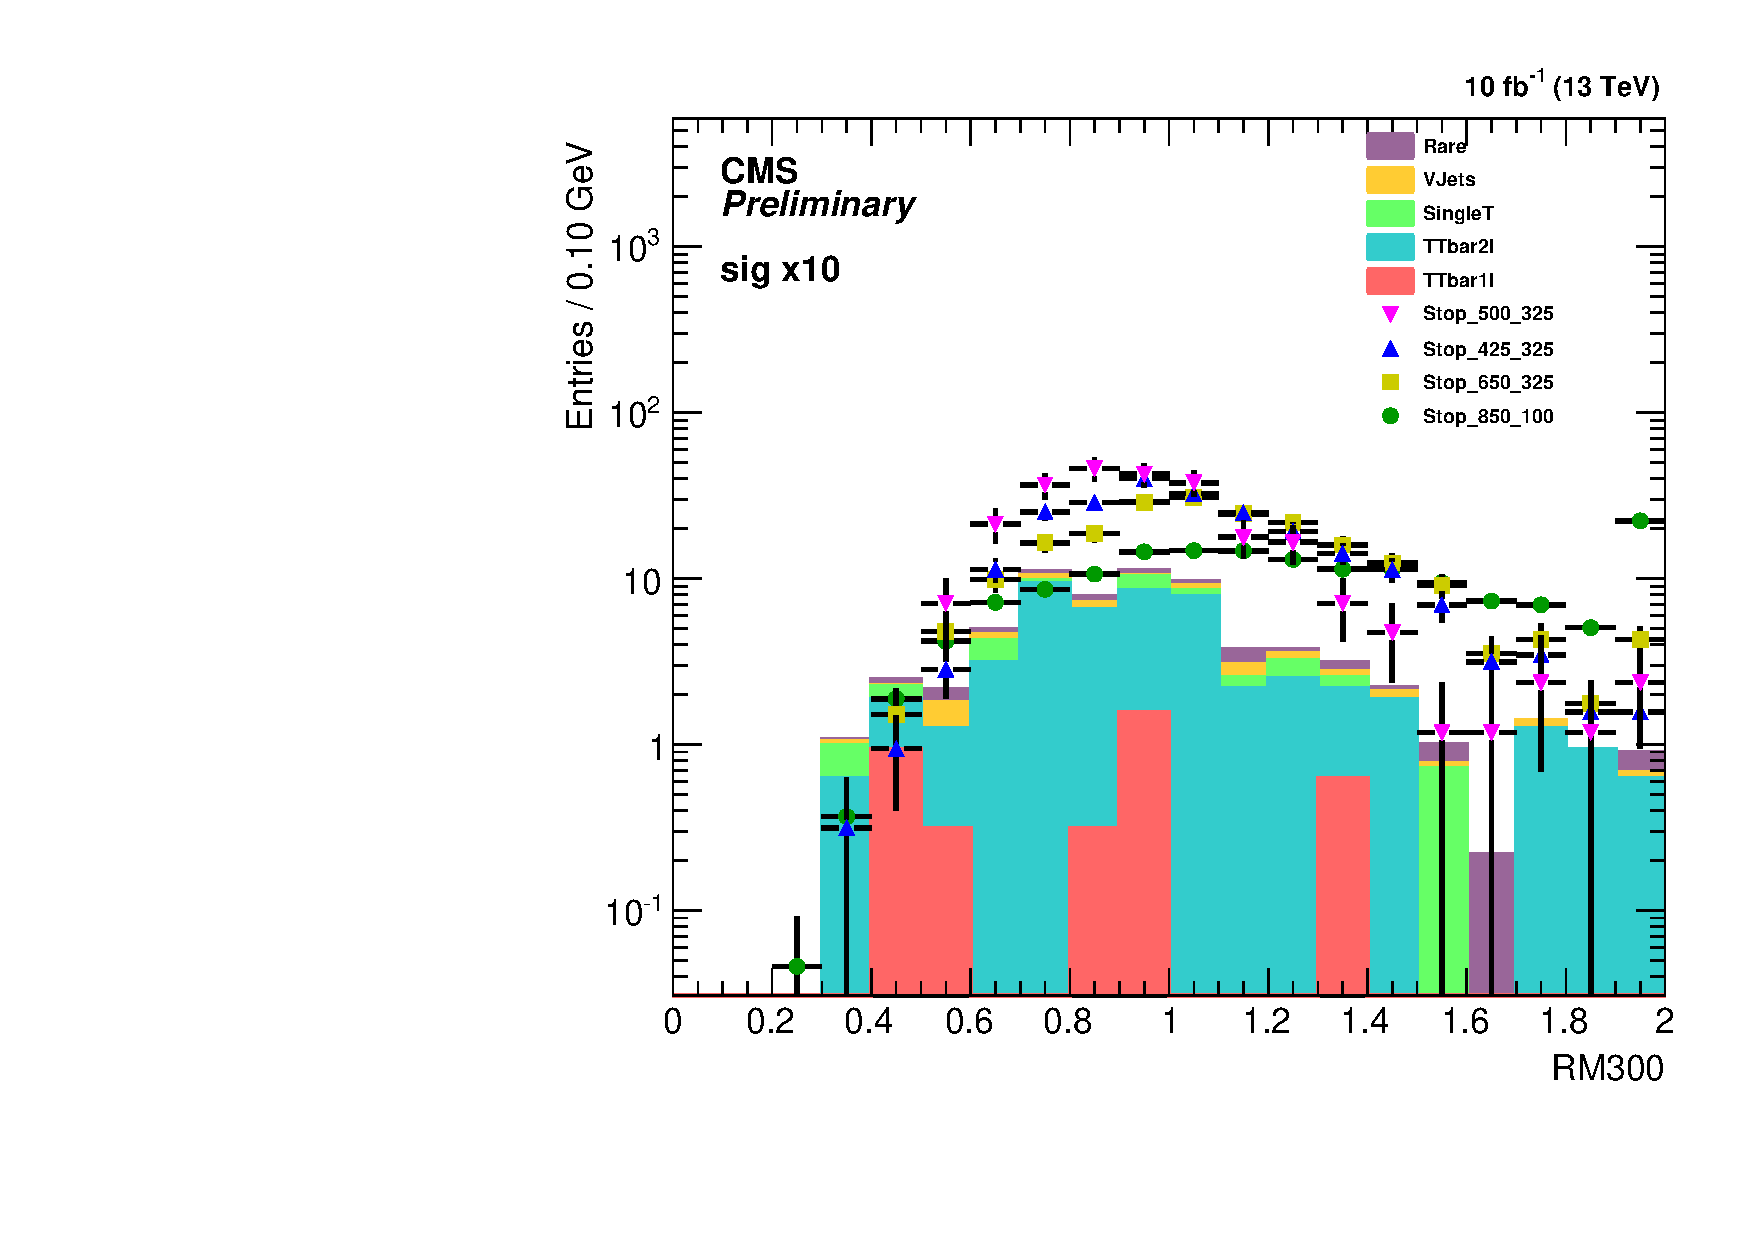
\includegraphics[width=0.49\textwidth]{Figures/SignalVariableStudies/RM300.pdf}
\label{fig:sigvarstudy:RMMTq:RM}
}
\subfigure[$\MT(j_1,\MET)$ distribution.]{
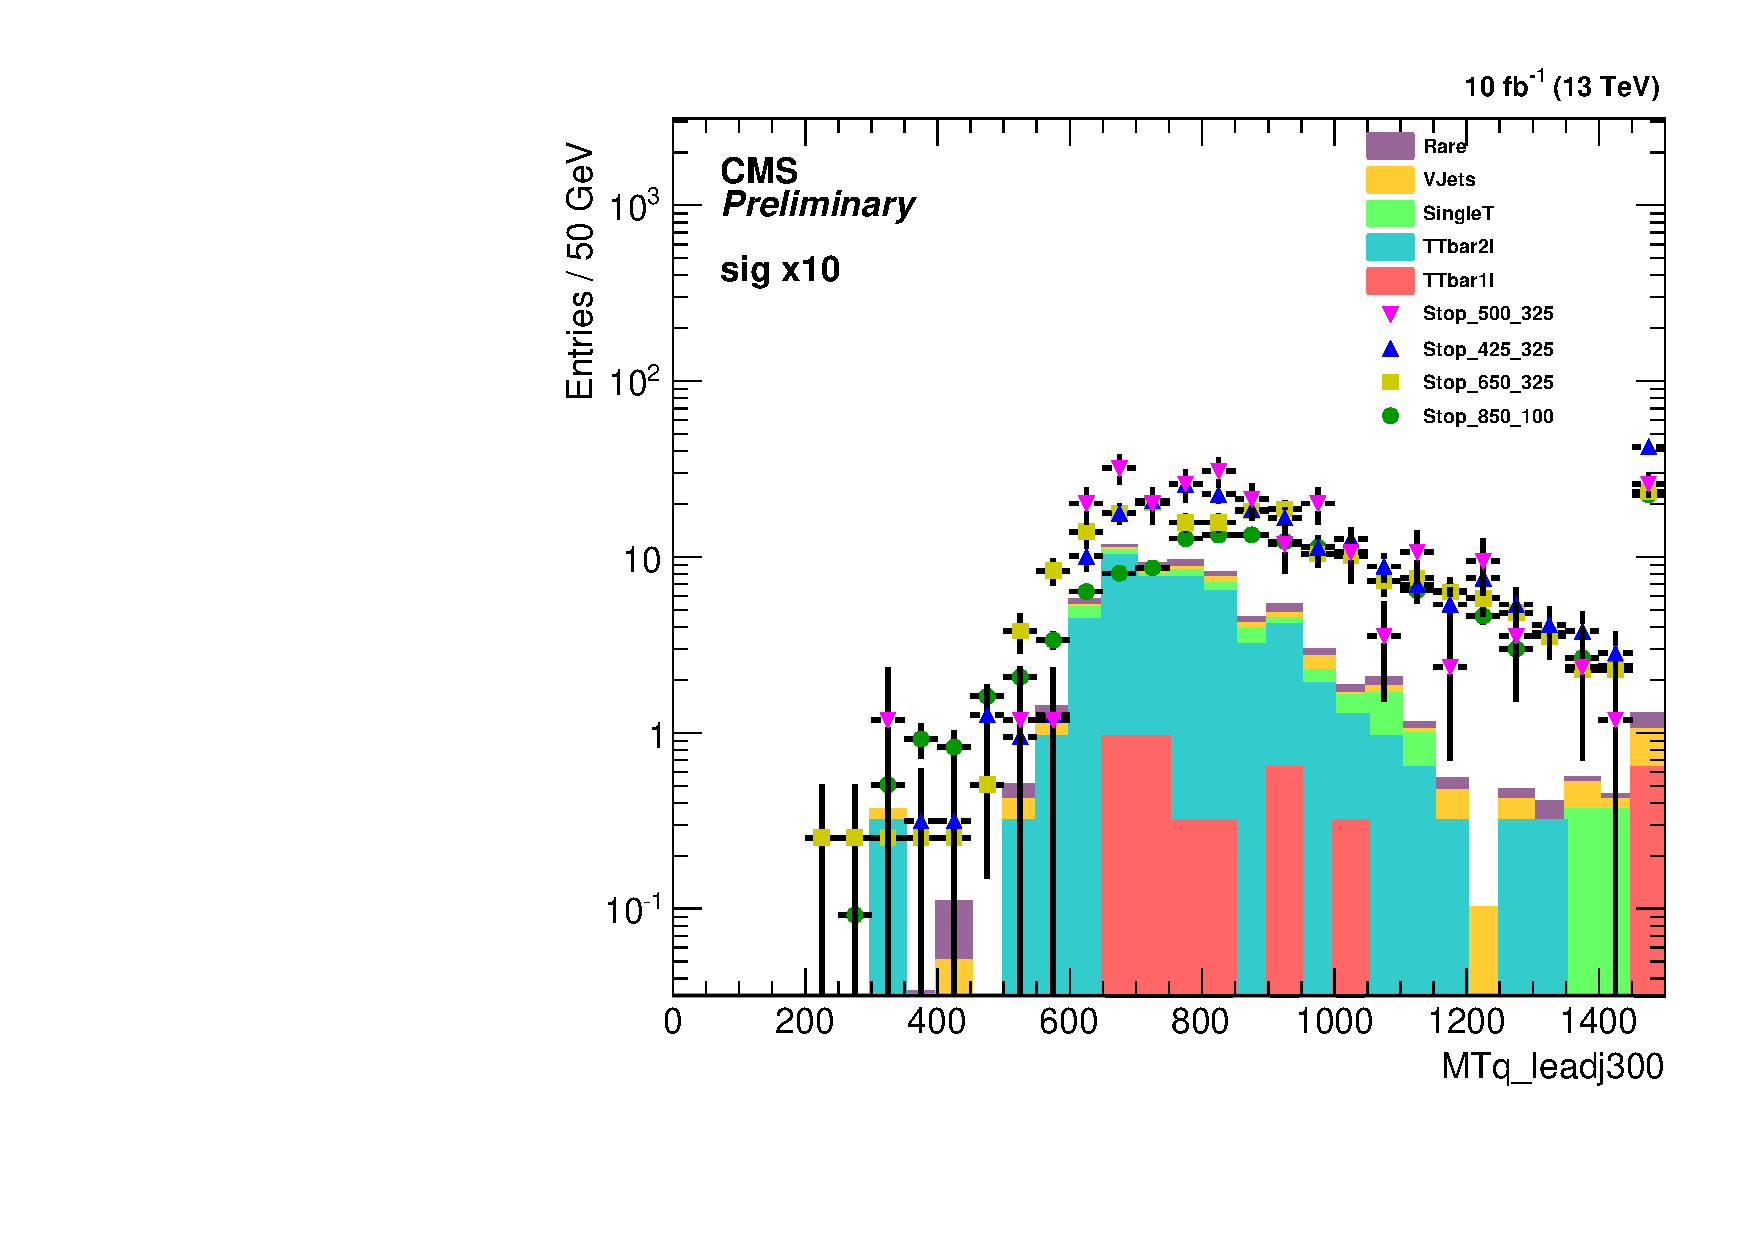
\includegraphics[width=0.49\textwidth]{Figures/SignalVariableStudies/MTq_leadj300.pdf}
\label{fig:sigvarstudy:RMMTq:MTq}
}
\caption{\label{fig:sigvarstudy:RMMTq} $R_M$ (left) and $\MT(j_1,\MET)$ (right) distributions.}
\end{figure}

\subsubsection{$\MT(j_1,\MET)$}

Similar to the motivation of $R_M$, the $\MT(j_1,\MET)$  variable targets the compressed spectra. Instead of a transverse momentum ratio, the transverse mass is computed:
\begin{equation}
\MT(j_1,\MET) = \sqrt{2\MET\pt^{j_1}(1-\cos\phi)},
\end{equation}
where $\phi$ is the angle between the \ptvec of the leading jet and \VEtmiss.
For the leading jet, we require $\pt>300\GeV$.

Figure~\ref{fig:sigvarstudy:RMMTq:MTq} shows the $\MT(j_1,\MET)$ distribution after preselection plus $\MET>300\GeV$. As a test selection $\MT(j_1,\MET)>750\GeV$ was chosen.

\subsection{Signal variable sensitivity for \texorpdfstring{$10\fbinv$}{10 fbinv}}
\label{sec:sigvarstudy:sensitivity}

As mentioned above, this study was performed under a slightly different preselection (especially regarding the second lepton veto) and under the assumption of a luminosity of 10\fbinv.
Therefore, the numbers quoted in this section should not be compared with any result of the main body. They rather serve as a relative comparison for the signal variables under study.

Several figures of merits were studied in this sensitivity study, among them simple S/B and S/$\sqrt{\mathrm{B}}$ checks, with S (B) being signal (background) yield of the signal region selected.
The one quoted here is the $Z_\mathrm{bi}$ variable~\cite{Cousins:2008zz}. We assume a relative background uncertainty of 30\% for this study.

As the preselection was found note to result a good sensitivity for any variable, we don't report its results here. For each variable, we quote numbers for the three other selections in table~\ref{tab:sigvarstudy:sensitivity}. The selection criteria on the variable under study was given in the respective subsections of section~\ref{sec:sigvarstudy:variables}.
%Quote Z_bi here, add the table of Zbis, mention those numbers are for 10/fbinv
\begin{table}[htb]
\begin{center}
\caption{\label{tab:sigvarstudy:sensitivity} Table for $Z_\mathrm{bi}$ values for the four signal mass hypothesis under three different event selections plus a selection on the variable under study. Its criteria is given in the respective subsections of section~\ref{sec:sigvarstudy:variables}.}
\small
\setlength{\tabcolsep}{2pt}
\begin{tabular}{|l|c|c|c|c|c|c|}
\hline
 & \multicolumn{3}{c|}{$M_{\PSQt} = 425\GeV$, $M_{\PSGczDo} = 325\GeV$} & \multicolumn{3}{c|}{$M_{\PSQt} = 500\GeV$, $M_{\PSGczDo} = 325\GeV$} \\
\hline
 Variable & $\MET> 300\GeV$ & $\chi^2_{\mathrm{had.}\cPqt} < 10$ & $\MTtW> 200\GeV$& $\MET> 300\GeV$ & $\chi^2_{\mathrm{had.}\cPqt} < 10$ & $\MTtW> 200\GeV$ \\
 \hline
 $t$ 											& 0.15 & 0.18 & 0.18			& -0.06 & -0.07 & -0.07\\
 $t_\text{mod}$ 									& -0.07 & -0.06 & -0.06		& -0.15 & -0.17 & -0.17\\
 $\MTtW$ 										& 0.16 & 0.20 & 0.20			& -0.03 & -0.02 & -0.02\\
 $\MTt(\ell\cPqb,\cPqb)$ 							& 0.12 & 0.16 & 0.16			& -0.02 & 0.02 & -0.04\\
 $\MTt(\ell\cPqb,\cPqb\cPq\cPq)$  					& 0.02 & 0.09 & 0.14			& -0.05 & -0.02 & -0.05\\
 $\MTt^{M_\mathrm{vis}=0}(\ell\cPqb,\cPqb)$ 			& -0.06 & -0.06 & -0.06		& -0.13 & -0.13 & -0.14\\
 $\MTt^{M_\mathrm{vis}=0}(\ell\cPqb,\cPqb\cPq\cPq)$	& -0.11 & -0.10 & -0.09		& -0.18 & -0.19 & -0.22\\
 $\MT(j_1,\MET)$ 								& 0.31 & 0.40 & 0.33			& 0.30 & 0.41 & 0.06\\
 $R_M$ 										& 0.27 & 0.35 & 0.34			& 0.26 & 0.34 & 0.13\\
 $\MTt(\ell,\cPq\cPq)$ 							& 0.01 & 0.06 & 0.04			& -0.07 & -0.03 & -0.12\\
 $\MTt^{M_\mathrm{vis}=0}(\ell,\cPq\cPq)$  			& -0.04 & -0.02 & -0.04		& -0.13 & -0.11 & -0.16\\
 \hline\hline
  & \multicolumn{3}{c|}{$M_{\PSQt} = 650\GeV$, $M_{\PSGczDo} = 325\GeV$} & \multicolumn{3}{c|}{$M_{\PSQt} = 850\GeV$, $M_{\PSGczDo} = 100\GeV$} \\
  \hline
 Variable & $\MET> 300\GeV$ & $\chi^2_{\mathrm{had.}\cPqt} < 10$ & $\MTtW> 200\GeV$& $\MET> 300\GeV$ & $\chi^2_{\mathrm{had.}\cPqt} < 10$ & $\MTtW> 200\GeV$ \\
 \hline
  $t$ 											& 0.66 & 0.78 & 0.78			& 0.48 & 0.57 & 0.57\\
  $t_\text{mod}$ 								& 0.90 & 1.04 & 1.01			& 0.68 & 0.79 & 0.78\\
  $\MTtW$ 									& 0.69 & 0.84 & 0.84			& 0.42 & 0.53 & 0.53\\
  $\MTt(\ell\cPqb,\cPqb)$ 							& 0.42 & 0.57 & 0.63			& 0.27 & 0.38 & 0.47\\
  $\MTt(\ell\cPqb,\cPqb\cPq\cPq)$  					& 0.20 & 0.32 & 0.51			& 0.16 & 0.32 & 0.58\\
  $\MTt^{M_\mathrm{vis}=0}(\ell\cPqb,\cPqb)$ 			& 0.55 & 0.66 & 0.76			& 0.40 & 0.47 & 0.61\\
  $\MTt^{M_\mathrm{vis}=0}(\ell\cPqb,\cPqb\cPq\cPq)$	& 0.55 & 0.70 & 0.89			& 0.38 & 0.51 & 0.76\\
  $\MT(j_1,\MET)$ 								& 0.22 & 0.31 & 0.42			& 0.16 & 0.23 & 0.48\\
  $R_M$ 										& 0.24 & 0.33 & 0.52			& 0.14 & 0.20 & 0.51\\
  $\MTt(\ell,\cPq\cPq)$ 							& 0.44 & 0.62 & 0.90			& 0.21 & 0.33 & 0.69\\
  $\MTt^{M_\mathrm{vis}=0}(\ell,\cPq\cPq)$  			& 0.45 & 0.62 & 0.91			& 0.22 & 0.33 & 0.68\\
 \hline
\end{tabular}
\end{center}
\end{table}

From this table we find the following: 

For the two mass points of larger mass splitting between the top squark and LSP masses, the most sensitive variable is the modified topness variable. Also good sensitivity is reached for the massless $\MTt(\ell\cPqb,\cPqb\cPq\cPq)$ variable, and the $\MTt(\ell,\cPq\cPq)$ variables. 
For the most sensitive variable we find the best separation without the \MTtW selection. 

For the two mass points with smaller mass splitting between the top squark and LSP masses, the most sensitive variables are the $R_M$ and $\MT(j_1,\MET)$ variables. The \MTtW and  $\MTt(\ell\cPqb,\cPqb)$, $\MTt(\ell\cPqb,\cPqb\cPq\cPq)$ variables also have some sensitivity, although the highest sensitivity is achieved before putting a selection on \MTtW.\\

This results need to be handled with care out of three reasons:
\begin{itemize}
\item Systematic/statistical uncertainties: In principle, the uncertainty value chosen can change the relative sensitivity. However, a relative background uncertainty of 10\% or 50\% the results are confirmed.
\item Total data yield: This numbers were obtained for 10\fbinv. For 2015 data we expect a data sample of 2-3\fbinv. These can change the conclusion significantly, as shown for one example below, when comparing topness versus \MTtW.
\item Simplified event selection: This study was performed with a single \MET selection of $\MET>300\GeV$. The final analysis has a \MET-binning approach with multiple signal regions along the \MET distribution. Depending on the correlation of the investigated variables and the \MET variable, this might lead to changes in the results. Also the $\chi^2_{\mathrm{had.}\cPqt}$ variable was calculated with a simplied jet energy resolution of 10\%.
\end{itemize}

One example, where these results did not agree with the strategy for 2015 data is shown in section~\ref{sec:sigvarstudy:MT2WvsTopness}.

\subsection{\texorpdfstring{\MTtW}{MT2W} versus (modified) topness}
\label{sec:sigvarstudy:MT2WvsTopness}

In figure~\ref{fig:sigvarstudy:MT2WvsTopness:ROC}, the ROC curves (signal efficiency versus background efficiency) for the two high mass points for the three variables \MTtW, and (modified) topness are compared.
\begin{figure}
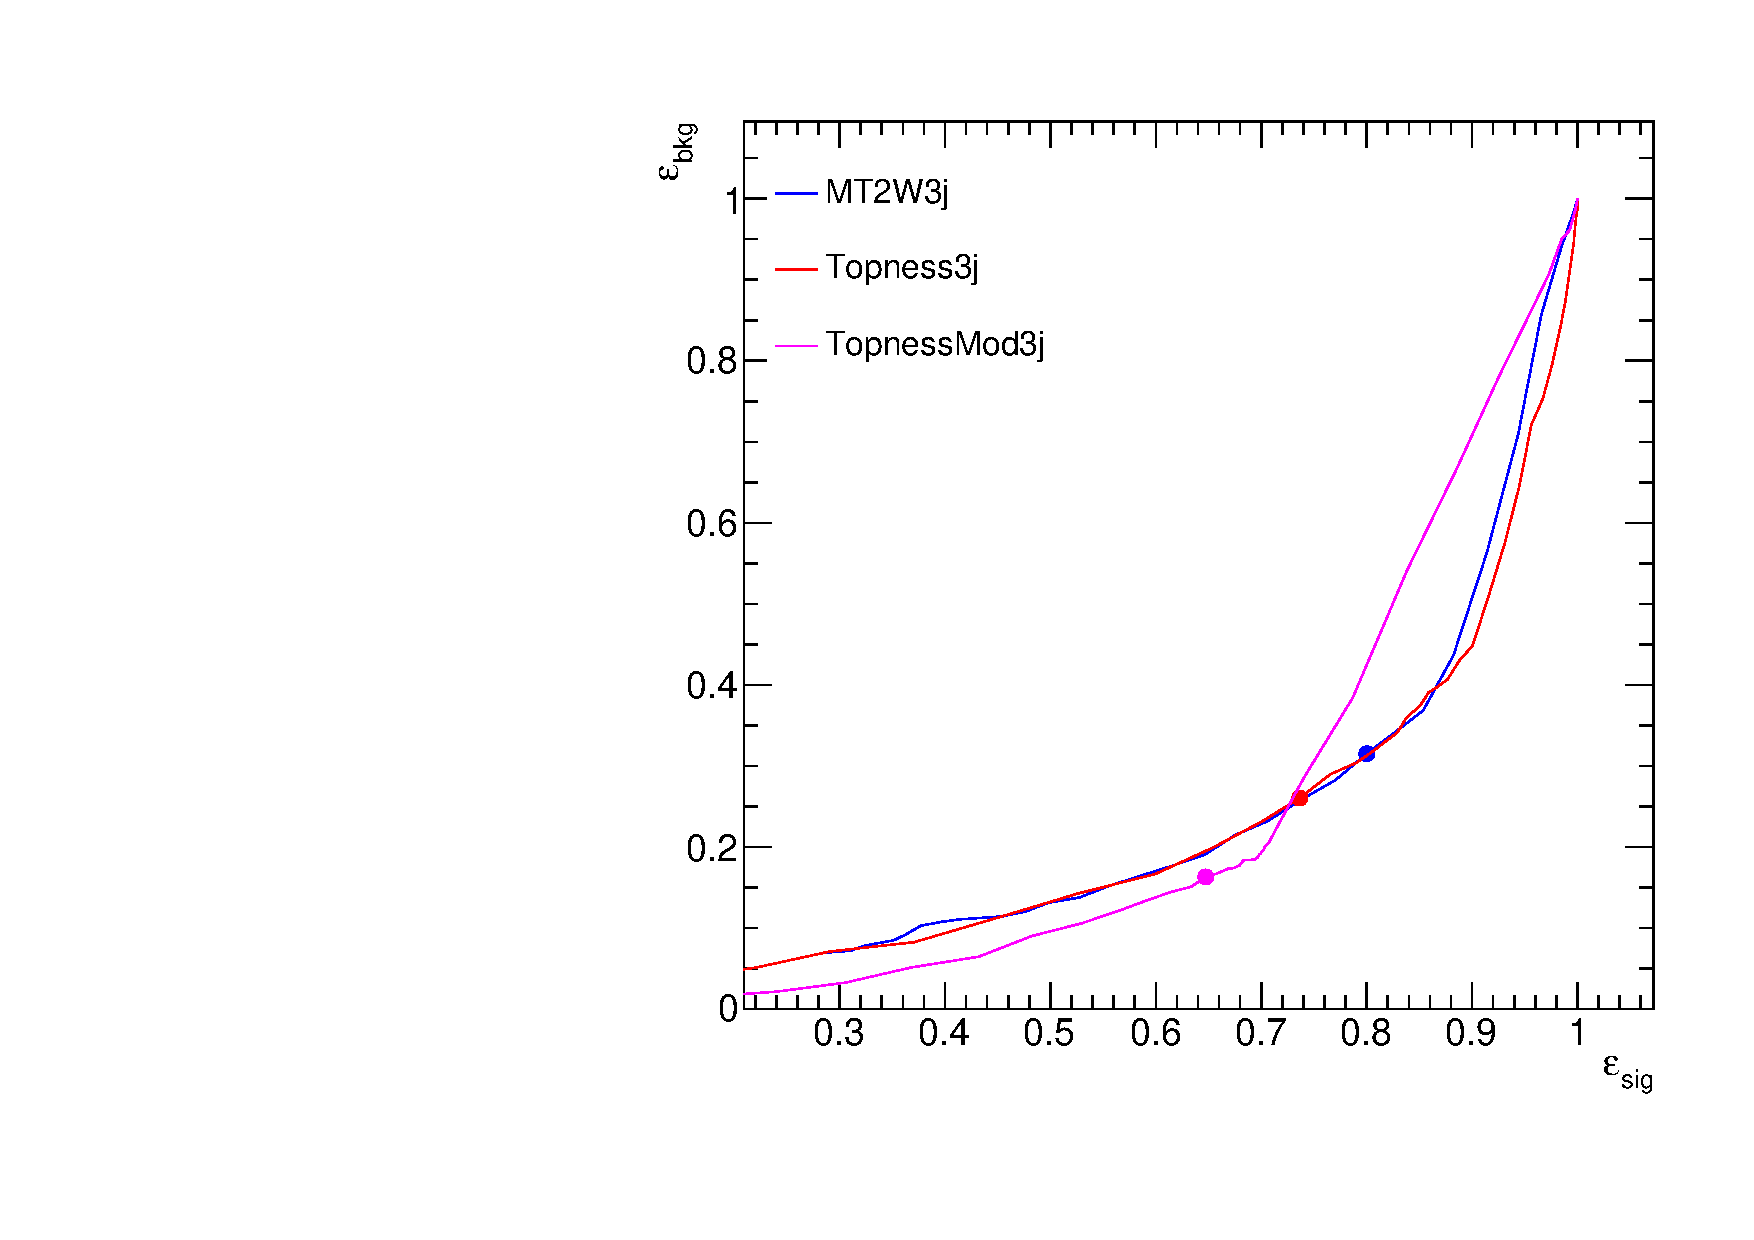
\includegraphics[width=0.49\textwidth]{Figures/SignalVariableStudies/ROC_j3Compare_Stop_850_100.pdf}
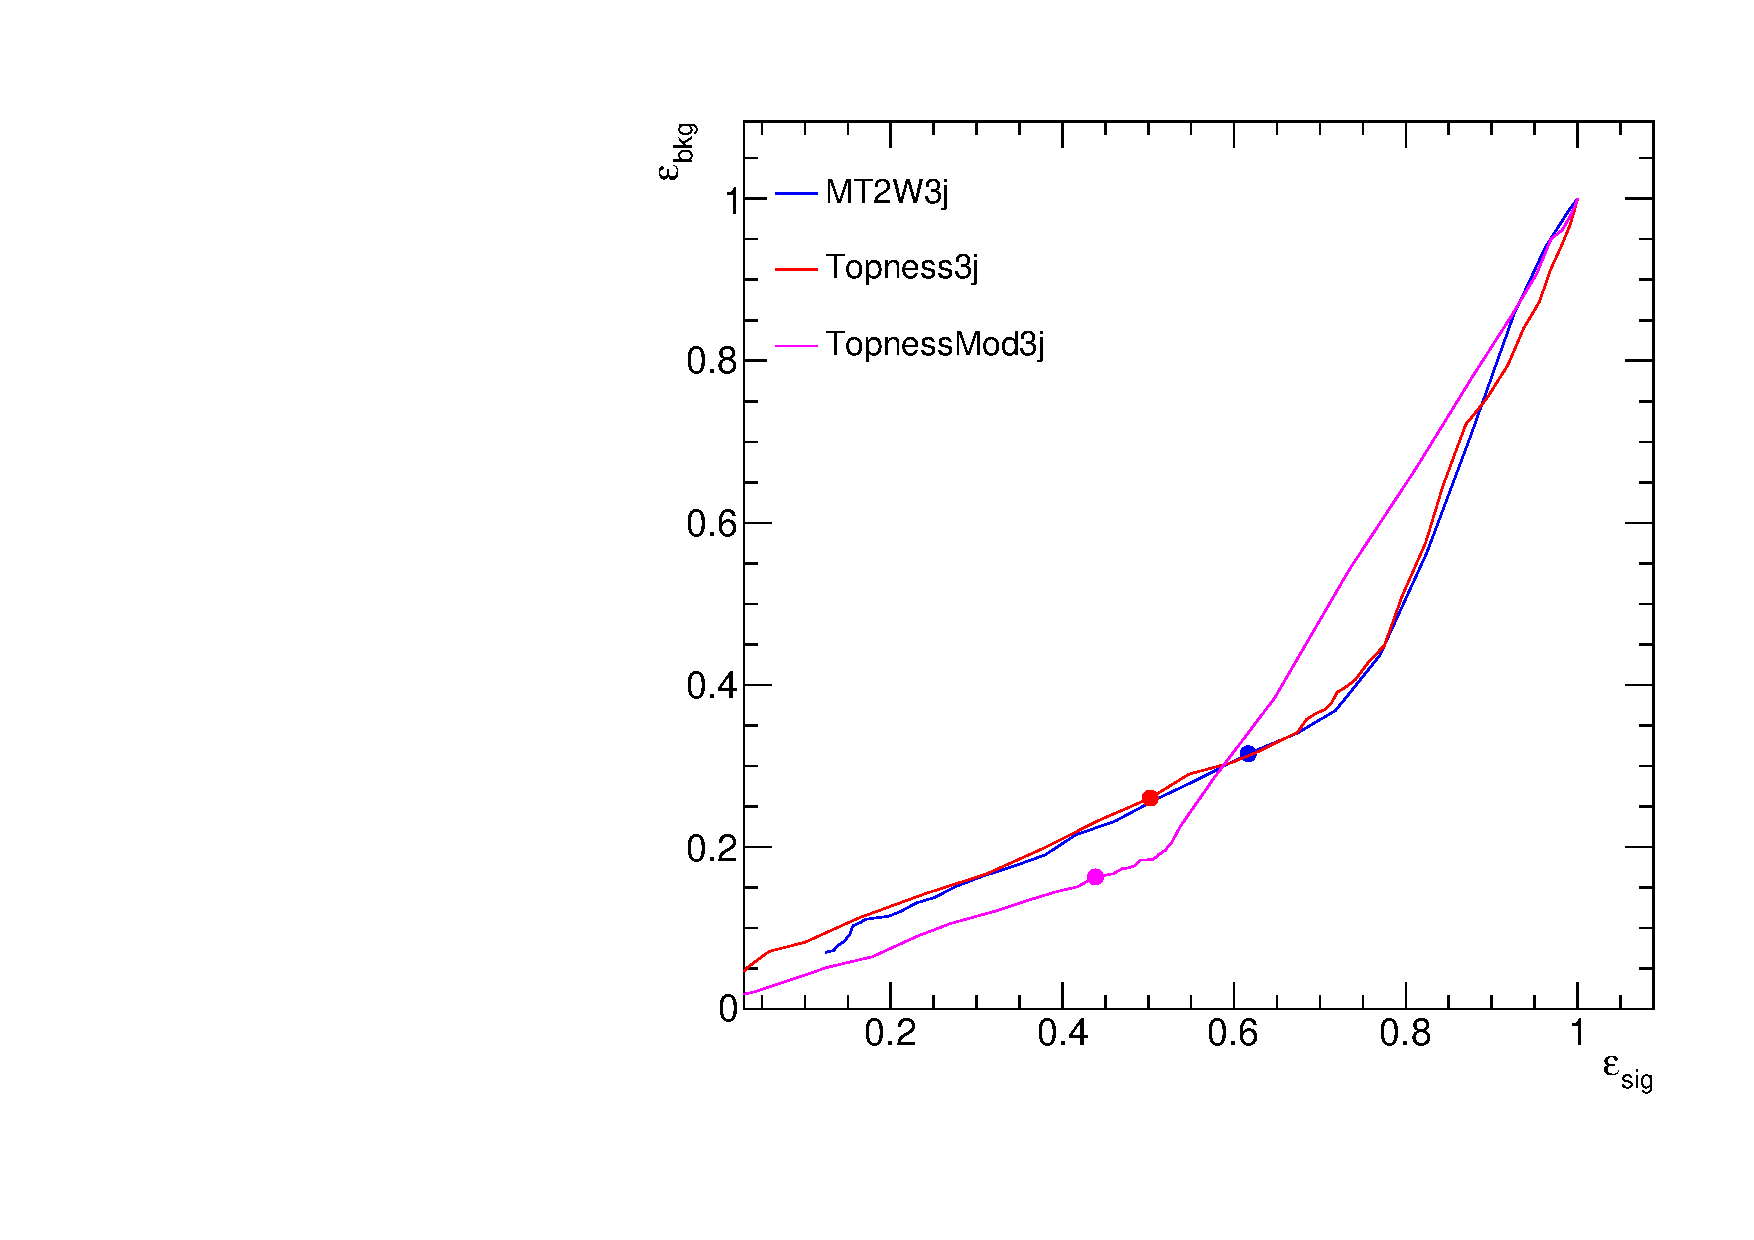
\includegraphics[width=0.49\textwidth]{Figures/SignalVariableStudies/ROC_j3Compare_Stop_650_325.pdf}
\caption{\label{fig:sigvarstudy:MT2WvsTopness:ROC} ROC curves for the floating \MTtW, and (modified) topness selection criteria for $M_{\PSQt} = 850\GeV$, $M_{\PSGczDo} = 100\GeV$ (left) and $M_{\PSQt} = 650\GeV$, $M_{\PSGczDo} = 325\GeV$ (right). The dots correspond to $\MTtW>200\GeV$ , $t> 9$, and $t_\mathrm{mod}> 7$.}
\end{figure}

The overall signal efficiency for the \MTtW selection is about 1/3 higher with respect to the modified topness selection.
We found, that already 5\fbinv, the significance ($Z_\mathrm{bi}$ value) reach an similar value, for less data, the \MTtW selection reaches higher values. Therefore, for the first round of this search with 2015 data, we chose to use the \MTtW variable as one signal variable.

When we accumulate more data, we will reevaluate this: We might either switch to the modified topness variable or choose to set harder selections on \MET.

A similar argument was found for the $R_M$ and $\MT(j_1,\MET)$  variables. The \MET selection already reduces the overall signal yield to small values for the lighter mass point signals. Thus, an additional selection on those variable decrease the signal yield, and do not result in a gain the overall signal sensitivity for the amount of data that will be selected in 2015.

\subsection{\texorpdfstring{\MET}{MET} versus \texorpdfstring{$\MET\sqrt{\HT}$}{MET/sqrt(HT)}}

Similar to the study in section~\ref{sec:sigvarstudy:MT2WvsTopness}, variants of the \MET variable were compared. One promising variable was $\MET\sqrt{\HT}$, where \HT is the scalar jet-\pt sum. Also a variant with \HT plus lepton-\pt was investigated. As figure~\ref{fig:sigvarstudy:METvsMETsqrtHT:ROC} shows, the plain \MET variable performs strongest.
\begin{figure}
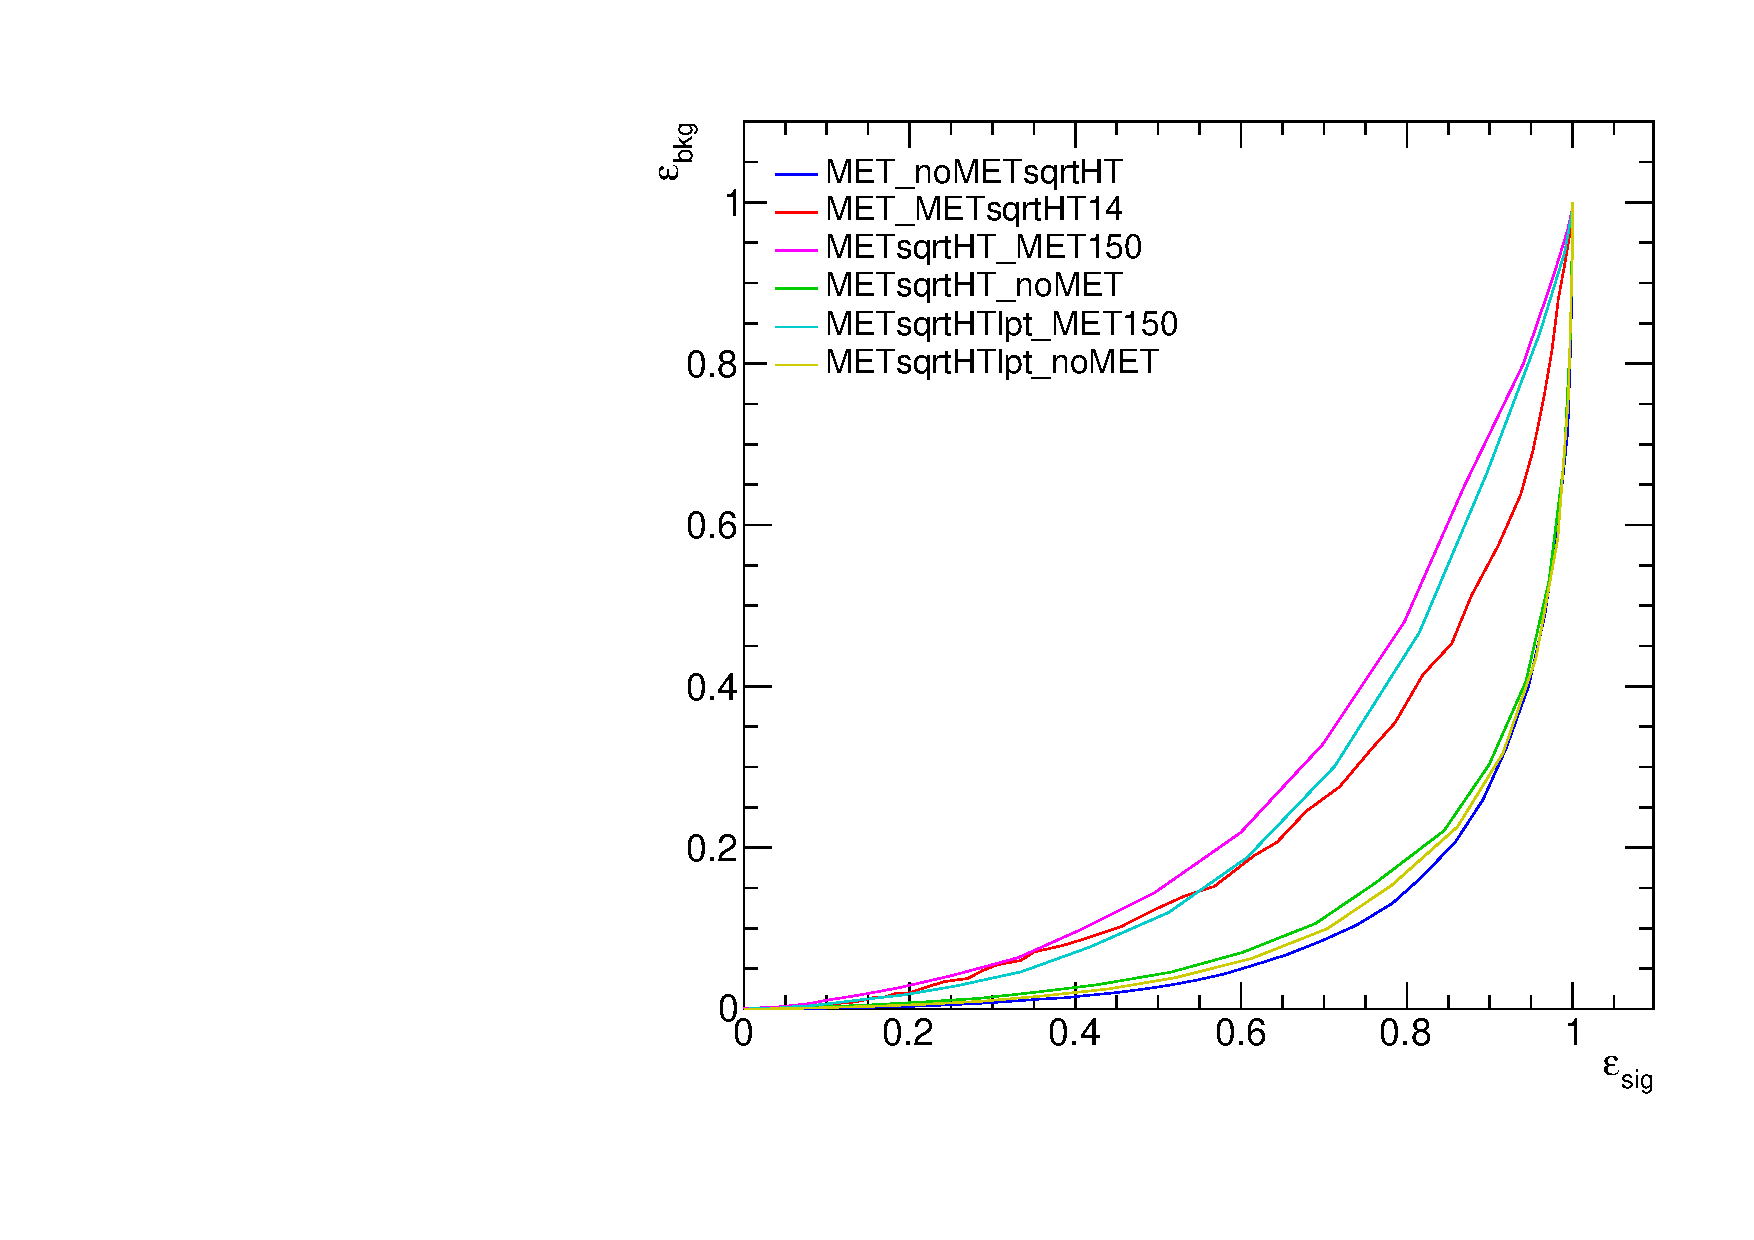
\includegraphics[width=0.49\textwidth]{Figures/SignalVariableStudies/ROC_METCompare_Stop_425_325.pdf}
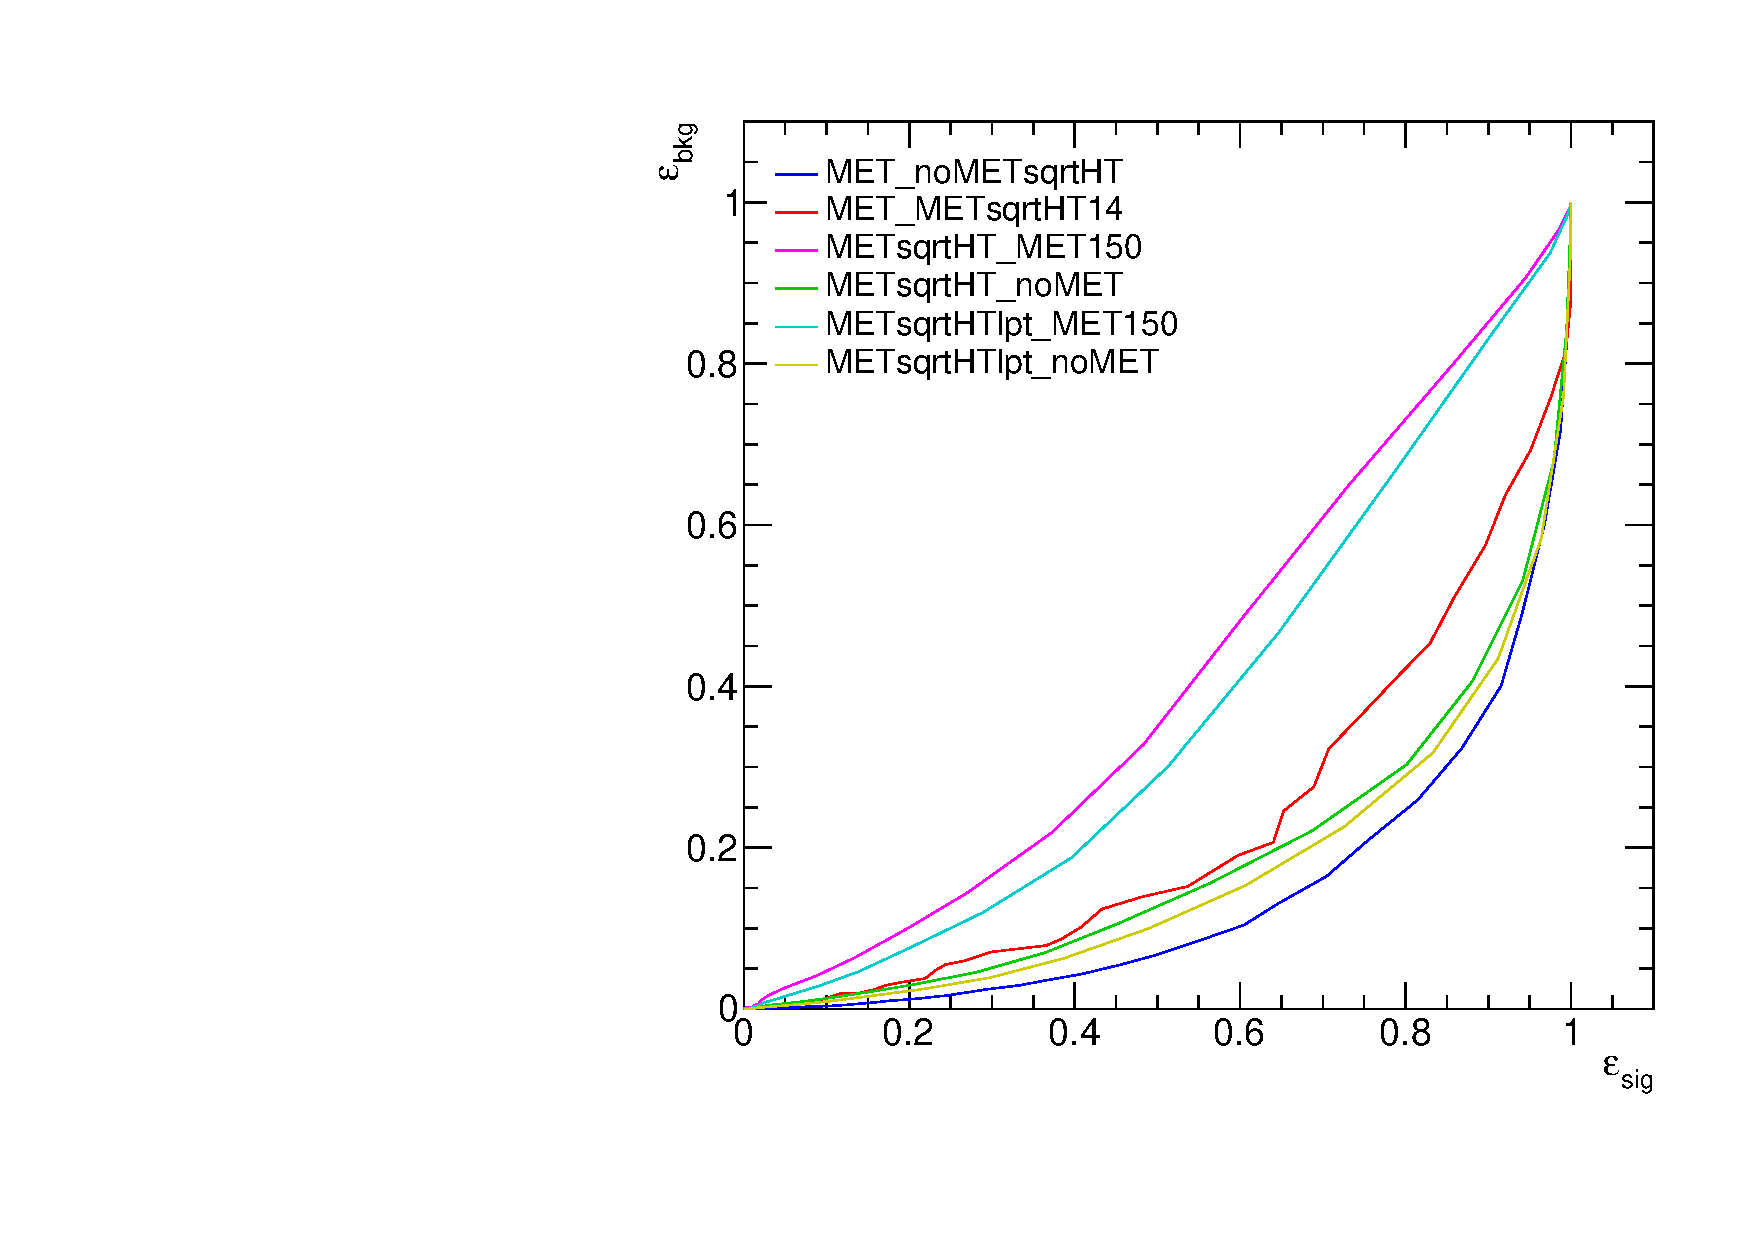
\includegraphics[width=0.49\textwidth]{Figures/SignalVariableStudies/ROC_METCompare_Stop_500_325.pdf}
\caption{\label{fig:sigvarstudy:METvsMETsqrtHT:ROC} ROC curves for the floating \MET, $\MET\sqrt{\HT}$ and $\MET\sqrt{\HT+\ell\text{-}\pt}$ criteria for $M_{\PSQt} = 425\GeV$, $M_{\PSGczDo} = 325\GeV$ (left) and $M_{\PSQt} = 500\GeV$, $M_{\PSGczDo} = 325\GeV$ (right). The various curves are more separated for the two higher signal mass points.}
\end{figure}

The studies of this appendix led to the signal region definitions of \MET and \MTtW as described in section~\ref{sec:obj_sel:signal_regions}.

\subsection{Discussion}

Even for 5\fbinv, the topness or modified topness variable don't increase the significance with respect of the usage of the \MTtW variable. The \MTt variable results in a greater background rejection for a working point with high signal efficiency. The modified topness variable, on the other hand, has a superior background rejection when choosing a working point with low signal efficiency.
Therefore, for an analysis of a large data sample ($>10\fbinv$), one might consider changing the selection of \MTtW to modified topness. However, as other variables will also play a role, a definite answer cannot be given at this stage of the analysis.

For compressed signals, we saw that both $R_M$ and $\MT(j_1,\MET)$ can improve the signal efficiency. As it was shown above {\color{red} ADD REFERENCE TO DANS STUDY}, for the current data sample, a simple selection on the leading jet-\pt is the most efficient selection one can do. The additional information in $R_M$ or $\MT(j_1,\MET)$ does not bring a large gain so far.





\section{Signal variable studies for T2tb and T2bW like signatures}
\label{sec:sigvarstudy2}

\emph{Please note: that this study has been performed under the assumption of 3\fbinv. Final studies (SEE DISCUSSION) led to the conclusion that for a datasample of 2\fbinv, there is no possibility to increase the significance including new signal variables, as such an additional binning leads to signal regions which have $\lesssim2$ signal events even with $\MET>250\GeV$.}

\emph{However, we include the discussion here for future reference.}

This appendix discusses investigations on various variables suitable for signal discriminating variables. As signal we have several mass points of top squark pair production where both top squark decays are $\PSQt\to\cPqb\PSGcpmDo$, $\PSGcpmDo\to\PW\PSGczDo$ (``T2bW''). We also obtimized this including signals where we have a mixture of the decay mentioned above and decays like $\PSQt\to\cPqt\PSGczDo$ (``T2tb'').
For defining event selections, we considered signal region selection sensitive to all three modes (T2tt, T2tb, and T2bW).

Therefore, the above discussion of section~\ref{sec:sigvarstudy} is valid here, and won't be repeated.

The event selection for this study is the same as the one quoted in section~\ref{sec:sigvarstudy:evtselection}, with the exception that we use the proper second lepton veto (including isolated track and tau vetos) of the analysis, see section~\ref{sec:obj_sel:lepton_sel}.

\subsection{Signal variables under study}
\label{sec:sigvarstudy:variables2}

\subsubsection{$M_{\ell\cPqb}$}

The invariant of the lepton--b-jet pair coming from the same top quark decay should, for perfect resolution, have an endpoint at $M_{\ell\cPqb} \approx 153\GeV$. For a T2bW-like signature, this bound does not exist. In fact the bound for a T2bW-like signature will be at 
\begin{equation*}
M_{\ell\cPqb} = M(\PSQt_1) \left(1-\frac{M^2(\PSGcpmDo)}{M^2(\PSQt_1)}\right)
\end{equation*}

Therefore, this variable could greatly reduce the background for dileptonic $\cPqt\cPaqt+$jets.

Figure~\ref{fig:sigvarstudy:MlbDRlb:Mlb} shows the $M_{\ell \cPqb}$ distribution with the b-jet chosen to be the jet with the highest CSV discriminant. Other selections of the b-jet show virtually the same discrimination.

As it can be appreciated, for a T2bW-like signatures, most of the background is below $M_{\ell\cPqb} < 175\GeV$, thus this variable can potentially greatly increase the sensitivity for this signal.
As the T2tt-like signatures have a very similar distribution as the $\cPqt\cPaqt+$jets background, we always want to keep a selection, that also includes events with the low $M_{\ell\cPqb}$.

\begin{figure}
\subfigure[$M_{\ell \cPqb}$ distribution.]{
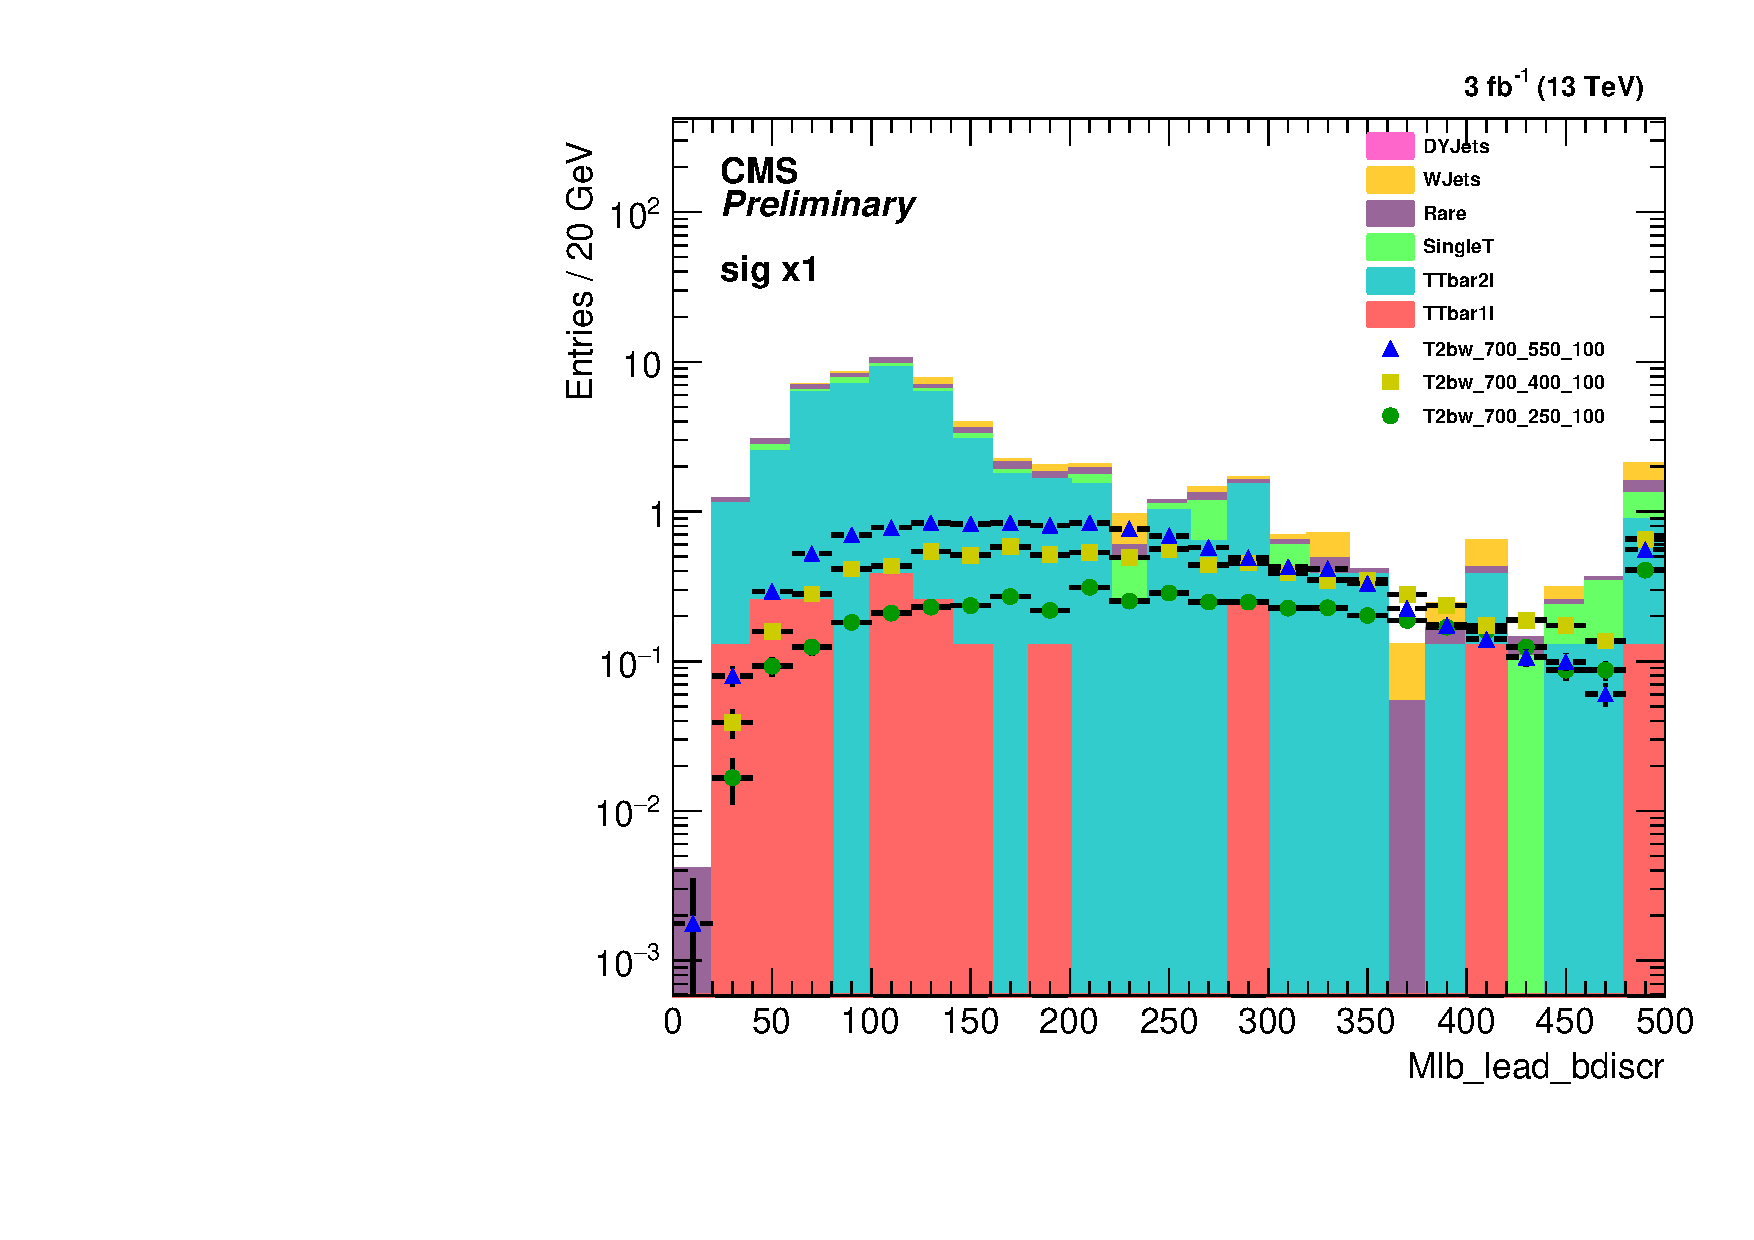
\includegraphics[width=0.49\textwidth]{Figures/SignalVariableStudies/Mlb_lead_bdiscr.pdf}
\label{fig:sigvarstudy:MlbDRlb:Mlb}
}
\subfigure[$\Delta R(\ell \cPqb)$ distribution.]{
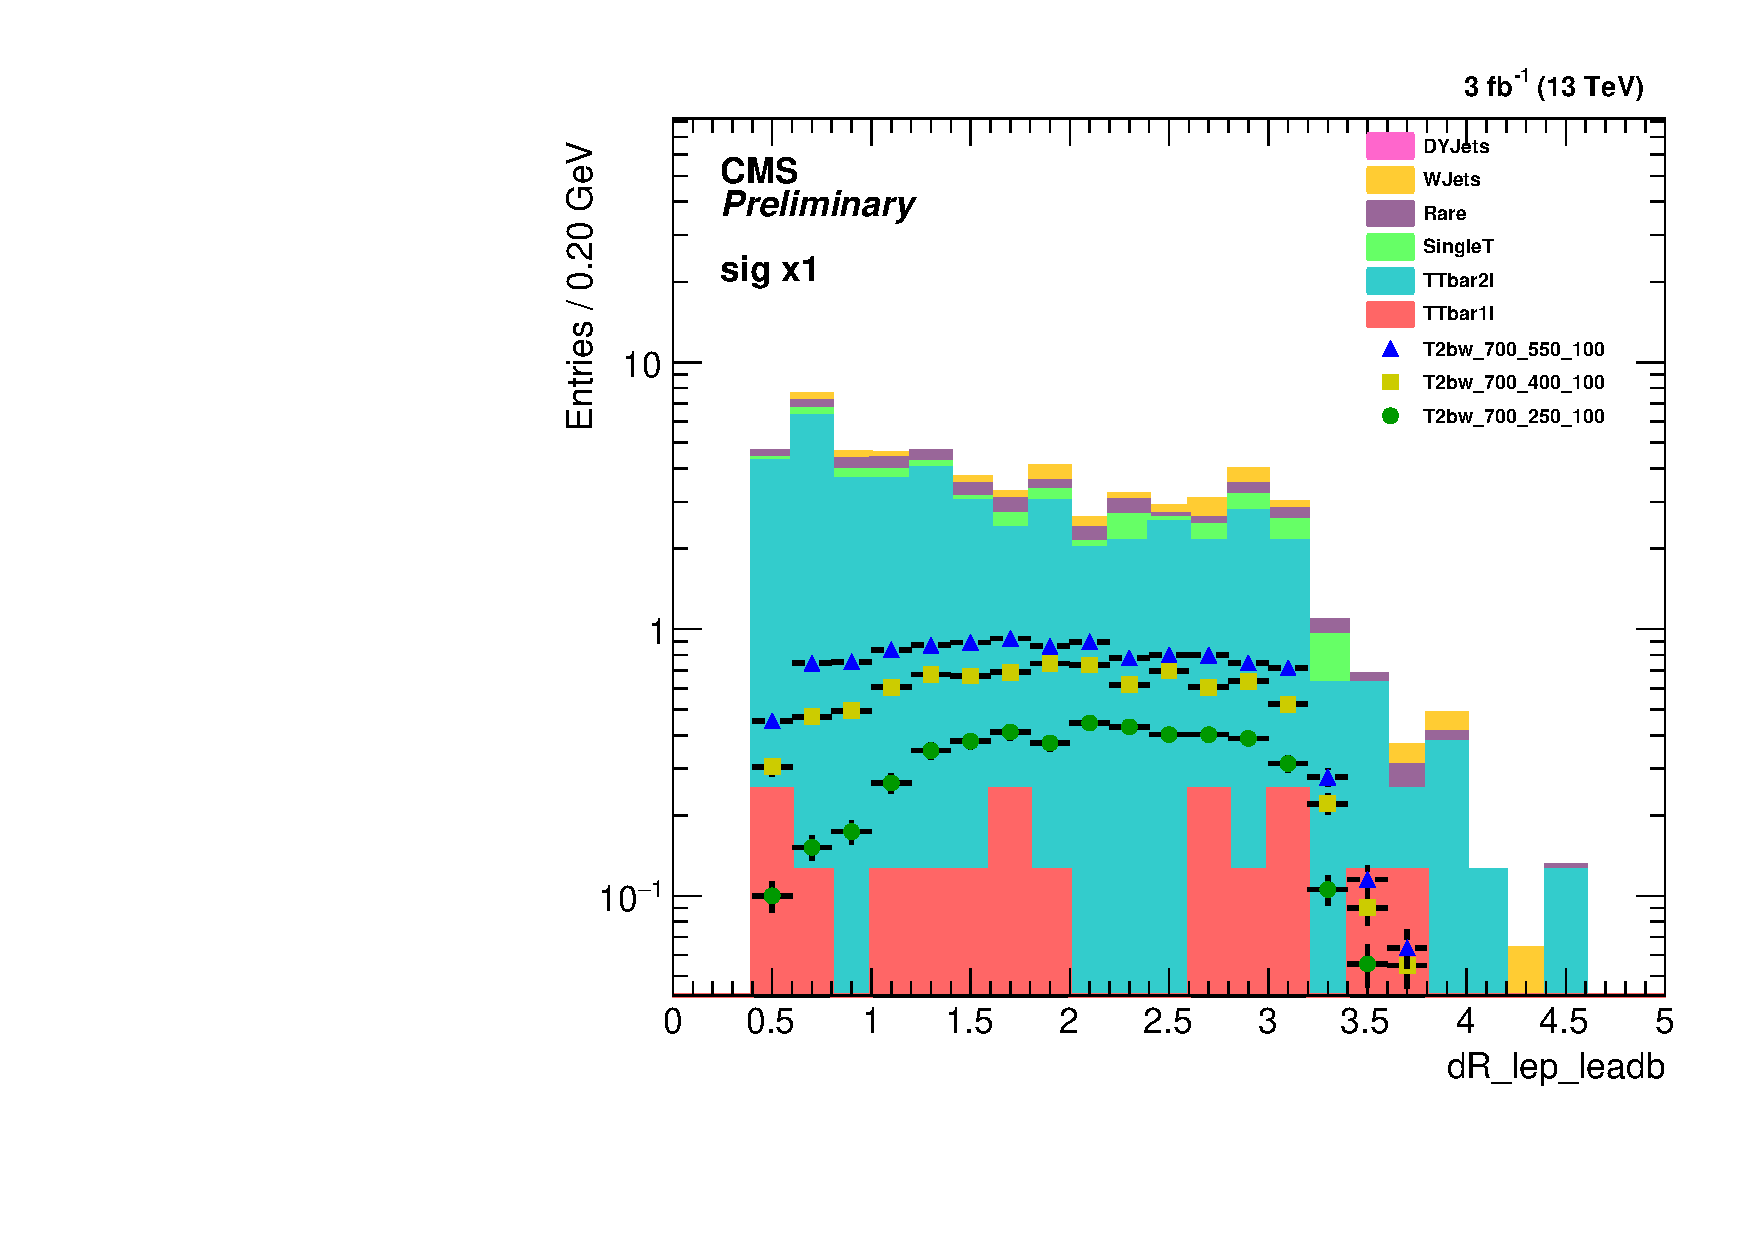
\includegraphics[width=0.49\textwidth]{Figures/SignalVariableStudies/dR_lep_leadb.pdf}
\label{fig:sigvarstudy:MlbDRlb:DRlb}
}
\caption{\label{fig:sigvarstudy:MlbDRlb} $M_{\ell \cPqb}$ (left) and $\Delta R(\ell \cPqb)$ (right) distributions.}
\end{figure}

\subsubsection{$\Delta R(\ell\cPqb)$}

In the 8 TeV analysis~\cite{Chatrchyan:2013xna}, $\Delta R(\ell\cPqb)$ had been used in the event selection.
The distribution of $\Delta R(\ell \cPqb)$ is shown in fig.~\ref{fig:sigvarstudy:MlbDRlb:DRlb}. We clearly see, that the discrimination is weaker. Maybe, this variable could be used in a multivariate analysis.

\subsubsection{Leading b-jet-\pt}

If the mass splitting between the top squark and the chargino is large, the b-jet produced in the top squark decay can be very boosted. In such a case, we expect great discrimination in the distribution of the leading b-jet-\pt. This is confirmed in fig.~\ref{fig:sigvarstudy:bptlpt:bpt}.

\begin{figure}
\subfigure[Leading b-jet-\pt distribution.]{
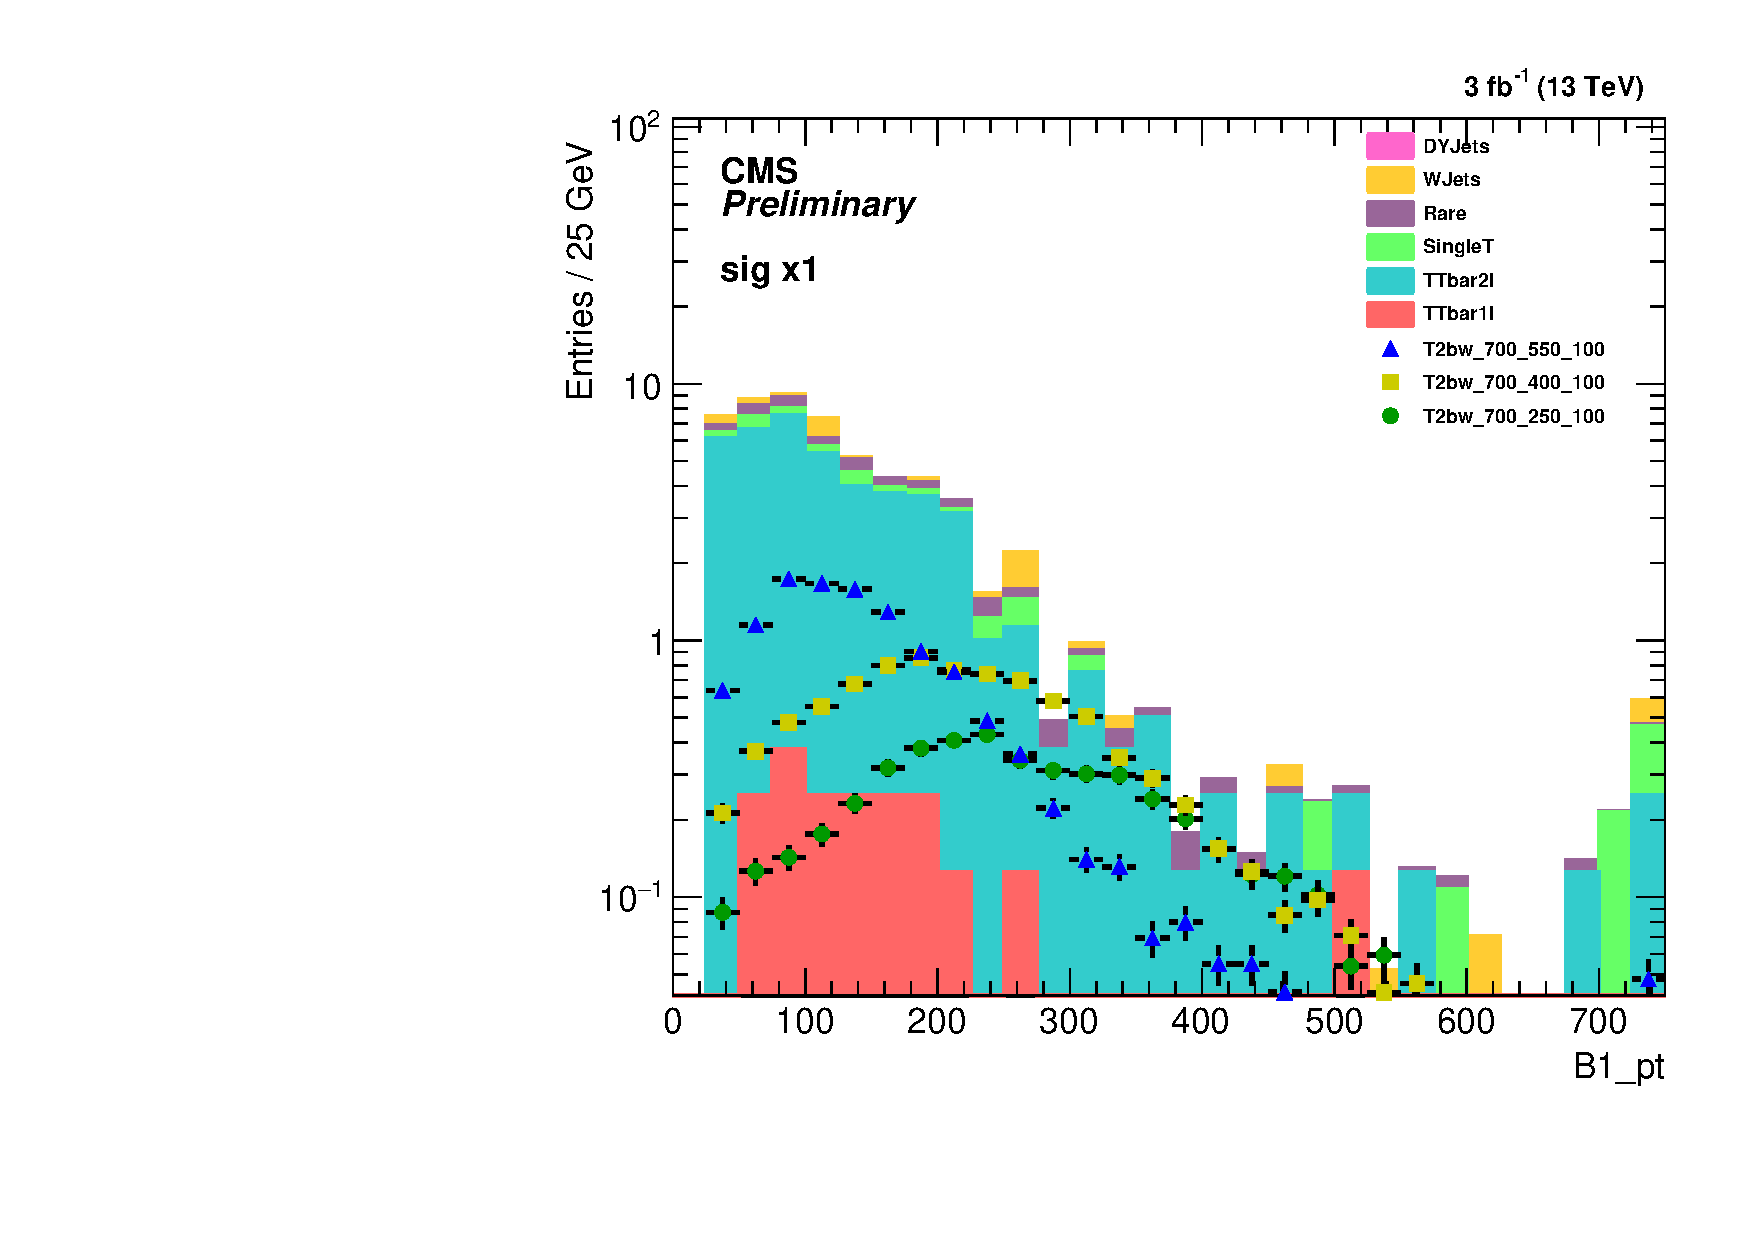
\includegraphics[width=0.49\textwidth]{Figures/SignalVariableStudies/B1_pt.pdf}
\label{fig:sigvarstudy:bptlpt:bpt}
}
\subfigure[:epton-\pt distribution.]{
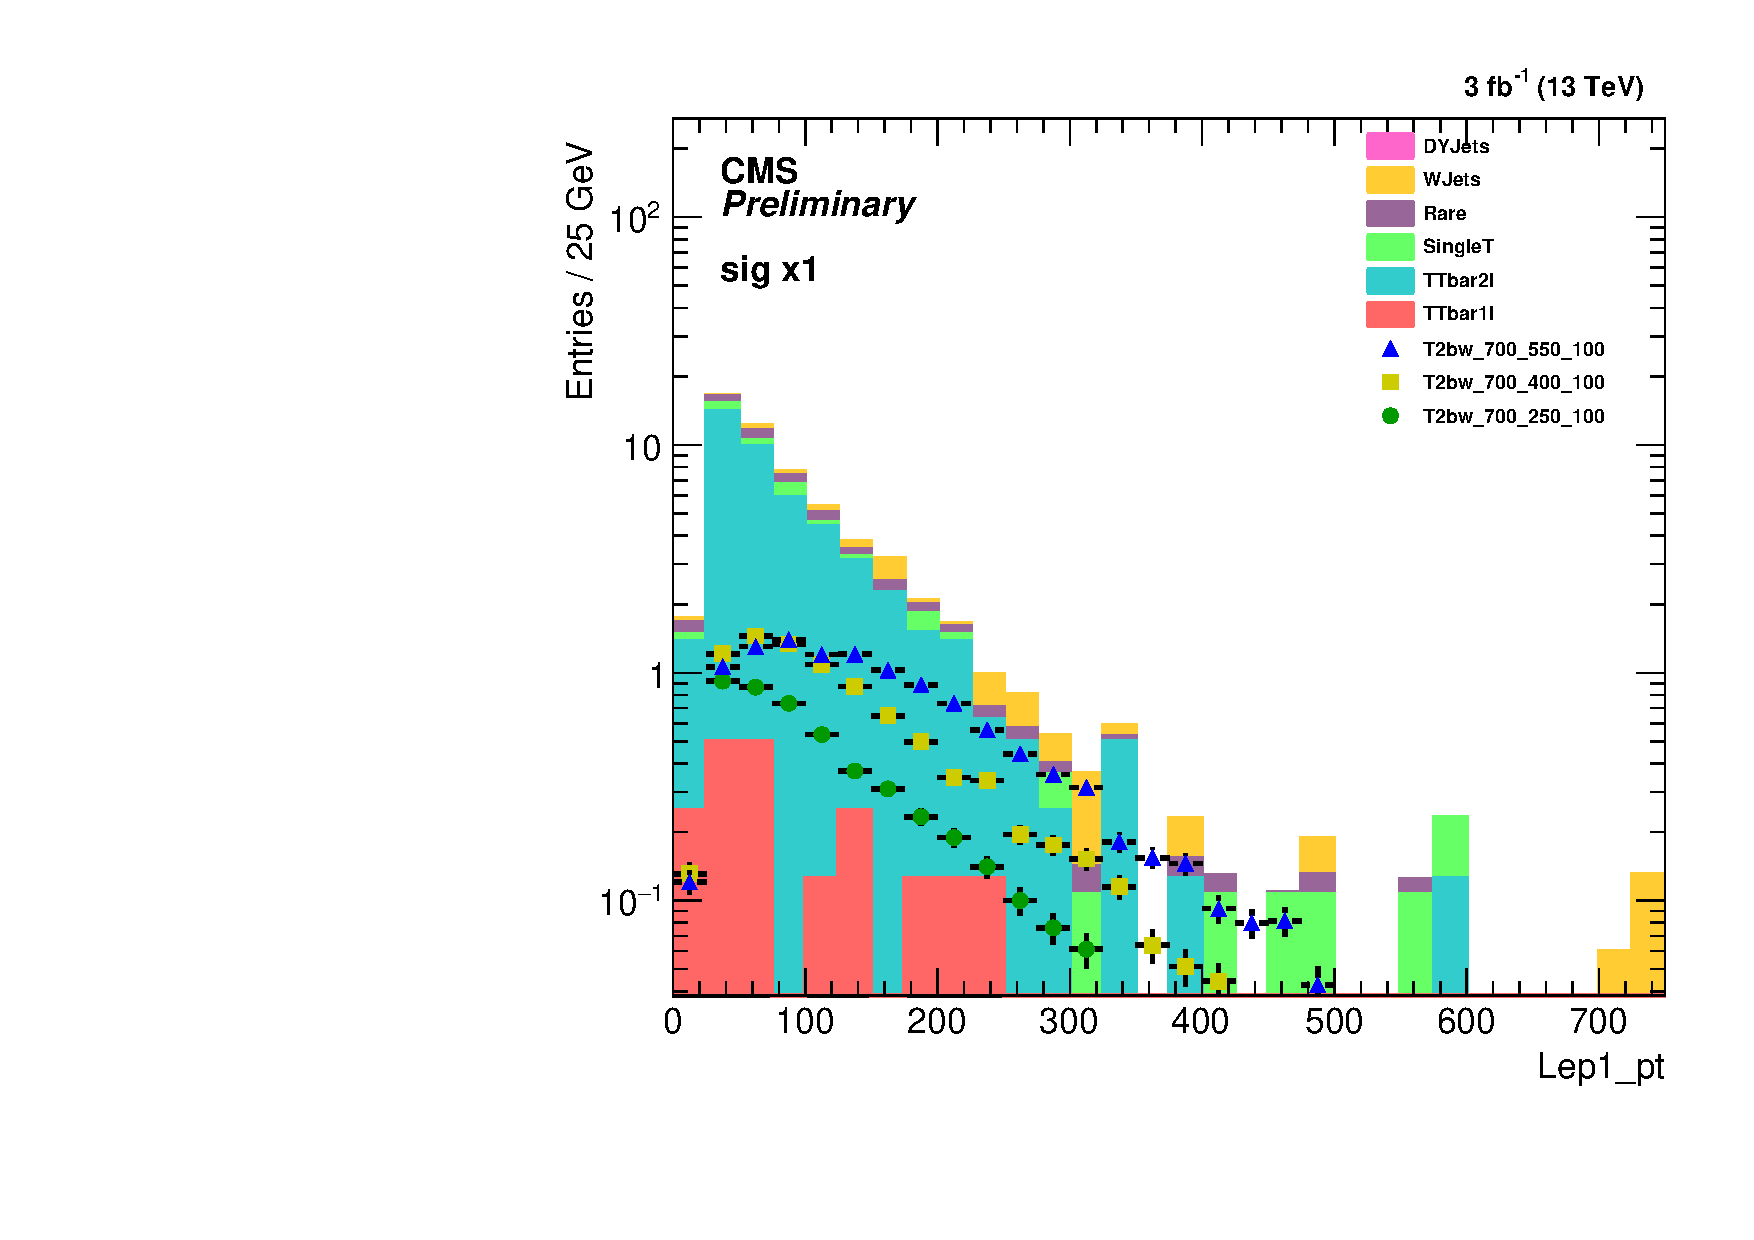
\includegraphics[width=0.49\textwidth]{Figures/SignalVariableStudies/Lep1_pt.pdf}
\label{fig:sigvarstudy:bptlpt:lpt}
}
\caption{\label{fig:sigvarstudy:bptlpt} Leading b-jet-\pt (left) and lepton-\pt (right) distributions.}
\end{figure}

\subsubsection{Lepton-\pt}

If the mass splitting between  the chargino and the LSP (in the top squark decay chain) is large, the lepton produced in the subsequent chargino can be very boosted, although the boost of the lepton depends on the momentum sharing between the lepton and neutrino of the \PW boson decay. Still, the lepton-\pt can enhance the signal discrimination, as it can be appreciated in fig.~\ref{fig:sigvarstudy:bptlpt:lpt}.

\subsubsection{$\MTt(\ell,\cPq\cPq)$}

Such a variable could be sensitive for the production of charginos as in $\PSQt\to\cPqb\PSGcpmDo$, $\PSGcpmDo\to\PW\PSGczDo$, as it should correlated with the mass splitting between the chargino and the LSP.

Figure~\ref{fig:sigvarstudy:MT2lqqHTfrac:MT2lqq} shows the $\MTt(\ell,\cPq\cPq)$ distribution. However, even for a T2bW like signature, no strong discrimination power was observed.

\begin{figure}
\subfigure[$\MTt(\ell,\cPq\cPq)$ distribution.]{
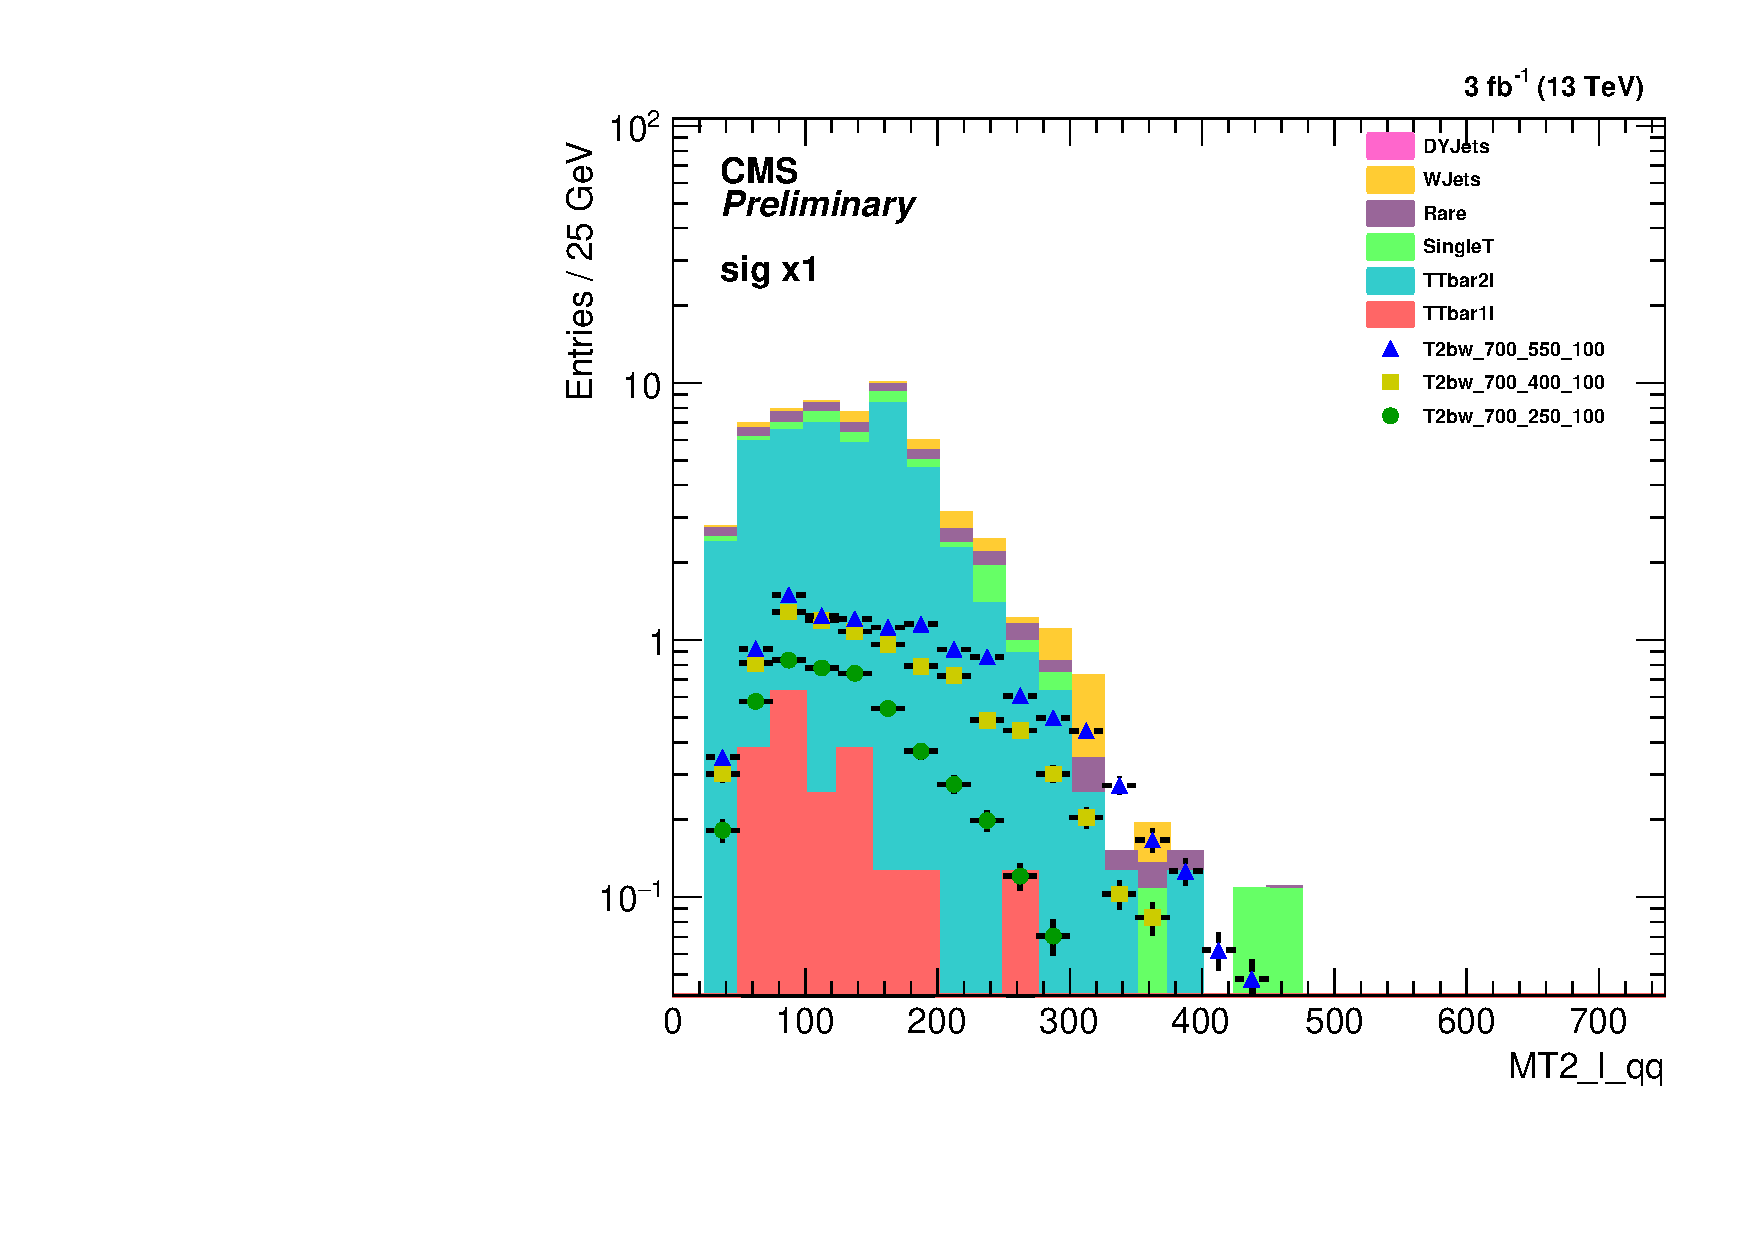
\includegraphics[width=0.49\textwidth]{Figures/SignalVariableStudies/MT2_l_qq_v2.pdf}
\label{fig:sigvarstudy:MT2lqqHTfrac:MT2lqq}
}
\subfigure[$\HT^\mathrm{frac}$ distribution.]{
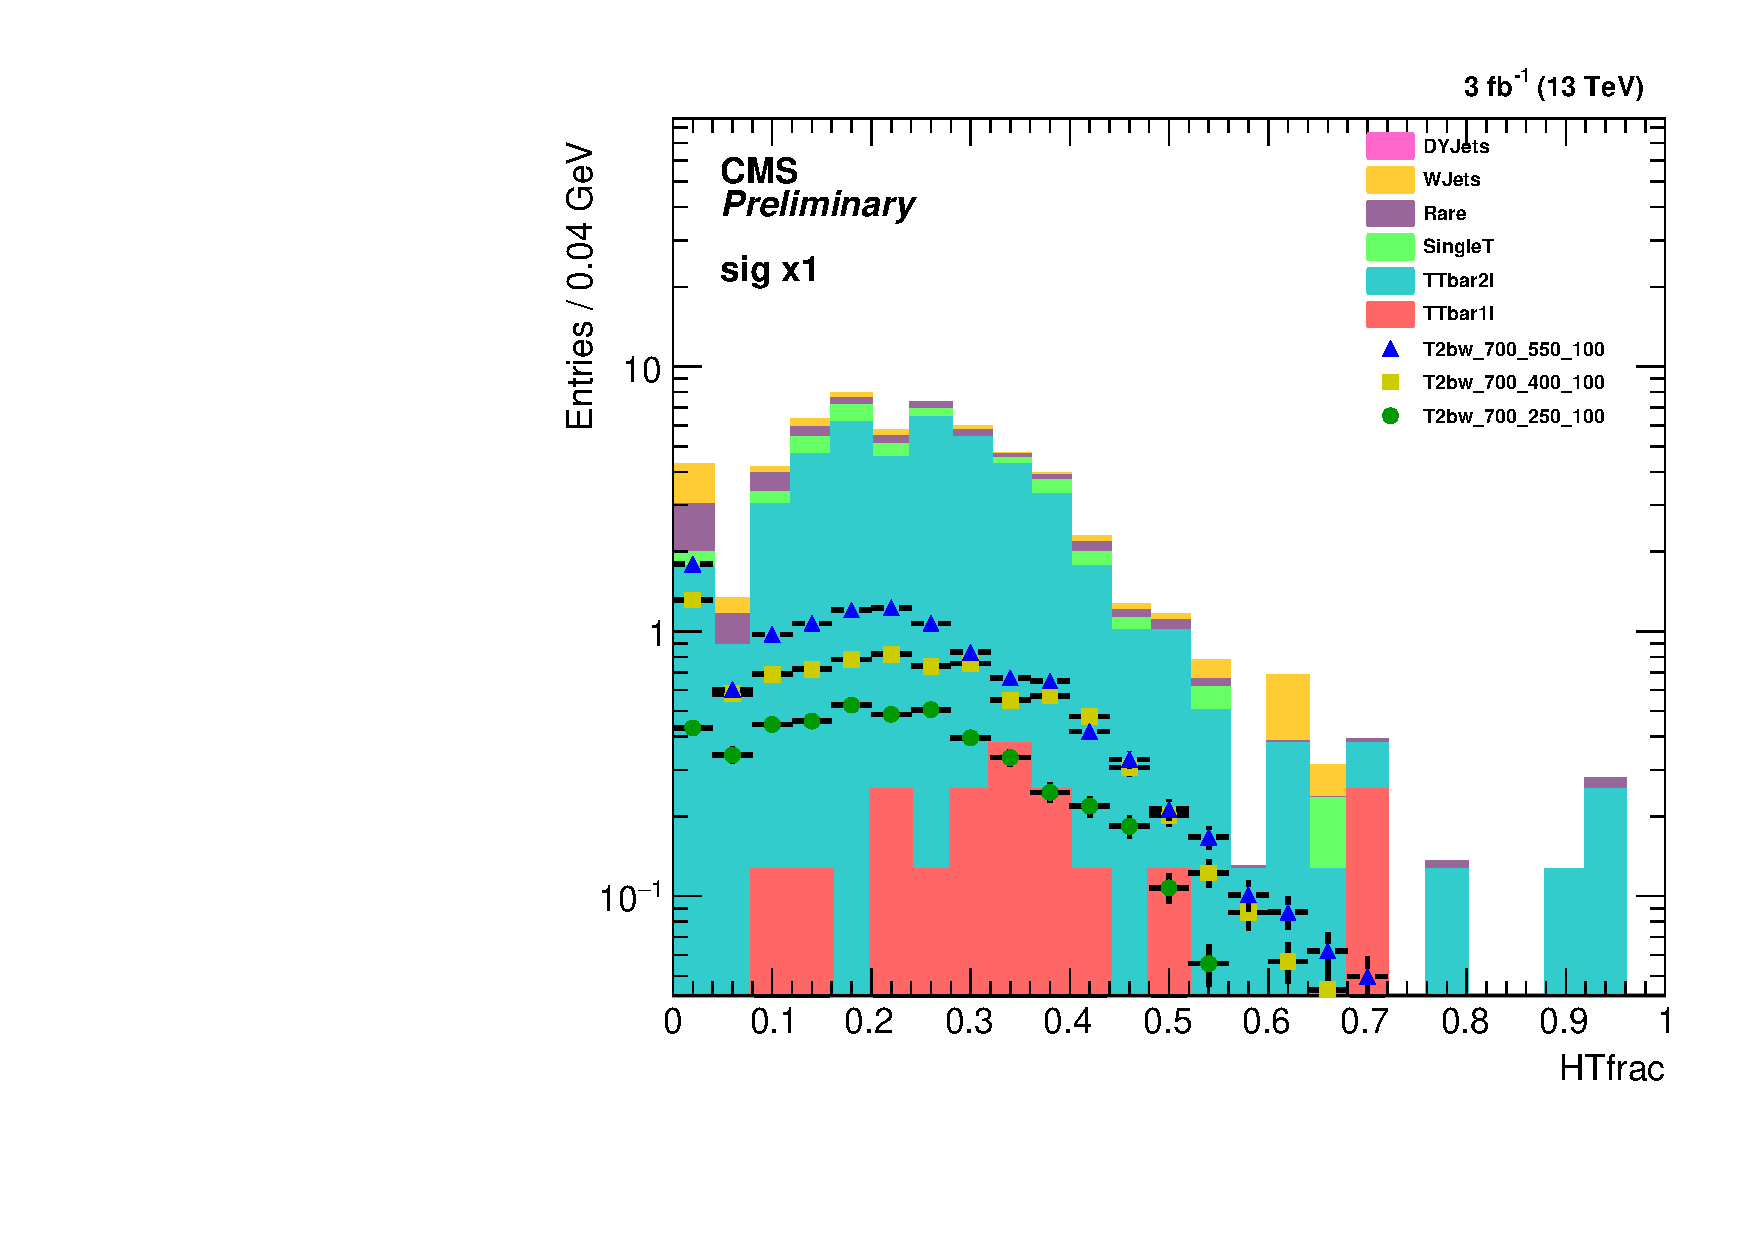
\includegraphics[width=0.49\textwidth]{Figures/SignalVariableStudies/HTfrac.pdf}
\label{fig:sigvarstudy:MT2lqqHTfrac:HTfrac}
}
\caption{\label{fig:sigvarstudy:MT2lqqHTfrac} $\MTt(\ell,\cPq\cPq)$ (left) and $\HT^\mathrm{frac}$ (right) distributions.}
\end{figure}

\subsubsection{$\HT^\mathrm{frac}$}

n the 8 TeV analysis~\cite{Chatrchyan:2013xna}, $\HT^\mathrm{frac}$ had been used in the event selection.
The corresponding distribution is shown in fig.~\ref{fig:sigvarstudy:MT2lqqHTfrac:HTfrac}. We clearly see, that the discrimination is very weak. Maybe, this variable could be used in a multivariate analysis.

\subsection{Evaluation of the signal variables}

From the variables studied, we found four main variables (besides \MET) that can enhance the signal--background discrimination: \MTtW, $M_{\ell \cPqb}$, the leading b-jet-\pt, and the lepton-\pt.

Already for 3\fbinv, we realized that for a ``cut-and-count'' analysis, the lepton-\pt is not suitable.
Also, adding two additonal variable selections on top of \MET and \MTtW is not feasible with 3\fbinv, although such a selection will be tempting with $\mathcal{O}(10\fbinv)$. However, that has to be studied.

Here, we summarize the study of adding either the leading b-jet-\pt or $M_{\ell \cPqb}$ to the selection, or even replacing \MTtW in the selection.
The procedure of the evalution was done as follows:
\begin{enumerate}
\item Define variables used. For \MTtW we chose a two-bin selection cutting at $\MTtW=200\GeV$, for $M_{\ell \cPqb}$ the value is at 175\GeV, while for the leading b-jet-\pt several options were investigated. It was found that cutting either at 100\GeV or 150\GeV are the best options for 3\fbinv.
\item Define a \MET binning for which we have $\gtrsim 2$ signal events in each bin at least one of the signal points.
\item Compute the signal sensitivity for all signals for that binning.
\item Get best ``averaged'' sensitivity for these signals. This last point is done subjectively, as we want to choose those signal regions that lead to good sensitivity for most of the signals, and avoid signal regions that lead to asymmetric sensitivities.
\end{enumerate}

With this procedure, 17 options were investigated. Following options seemed to be promising:
\begin{itemize}
\item v1: $\MTtW\lessgtr200\GeV$, up to 5 bins in \MET (8 bins)
\item v2: leading b-jet-$\pt \lessgtr 100\GeV$, $\MTtW\lessgtr200\GeV$, up to 4 bins in \MET (8 bins)
\item v3: leading b-jet-$b\pt \lessgtr 150\GeV$, $\MTtW\lessgtr200\GeV$, up to 3 bins in \MET (8 bins) 
\item v4: $M_{\ell \cPqb} \lessgtr 175\GeV$, $\MTtW\lessgtr200\GeV$, up to 3 bins in \MET (8 bins) 
\end{itemize}

The significances for all those options and all studies signal points is given in table~\ref{tab:sec:sigvarstudy:eval2}. For this table, all masses are given in GeV. Signals with $M(\PSQt_1) = 700\GeV$ have an LSP mass of 100 GeV, while signals with $M(\PSQt_1) = 600\GeV$ have an LSP mass of 50 GeV.

\begin{table}
\begin{center}
\caption{Significances for all those options and all studies signal points for 3\fbinv. All masses are given in GeV. Signals with $M(\PSQt_1) = 700\GeV$ have an LSP mass of 100 GeV, while signals with $M(\PSQt_1) = 600\GeV$ have an LSP mass of 50 GeV.\label{tab:sec:sigvarstudy:eval2}}
\tiny
%\setlength{\tabcolsep}{1pt}
%\scalebox{0.825}{
\begin{tabular}{|l|cccccc|ccc|cccc|}
\hline
signif & \multicolumn{6}{c|}{T2bW: $M(\PSQt_1)$-$M(\PSGcpmDo)$} & \multicolumn{3}{c|}{T2tb: $M(\PSQt_1)$-$M(\PSGcpmDo)$} & \multicolumn{4}{c|}{T2tt: : $M(\PSQt_1)$-$M(\PSGczDo)$} \\
   & 600-187.5 & 600-325 & 600-462.5 & 700-250 & 700-400 & 700-550 & 700-250 & 700-400 & 700-550 & 425-325 & 500-325 & 650-325 & 850-100 \\
\hline
v1 & 1.14 & 2.21 & 3.08 & 0.93 & 1.67 & 2.03 & 1.76 & 2.03 & 2.21 & 0.57 & 0.69 & 1.38 & 1.03\\ 
v2 & 1.29 & 2.32 & 3.06 & 1.00 & 1.72 & 1.99 & 1.71 & 1.99 & 2.12 & 0.52 & 0.57 & 1.38 & 0.94 \\
v3 & 1.35 & 2.32 & 3.09 & 1.08 & 1.79 & 2.04 & 1.79 & 2.05 & 2.19 & 0.48 & 0.54 & 1.39 & 0.98 \\
v4 & 1.34 & 2.35 & 3.14 & 1.08 & 1.83 & 2.13 & 1.73 & 2.01 & 2.15 & 0.54 & 0.66 & 1.41 & 0.95 \\
\hline
\end{tabular}
%}
\end{center}
\end{table}

For the assumption of 3\fbinv, the option v4 seemed overall most promising. The binning for that option as well as background and signal yields are given in tables~\ref{tab:sec:sigvarstudy:SR2} and~\ref{tab:sec:sigvarstudy:yields2}.

\begin{table}
\begin{center}
\caption{Binning for ``optimal'' signal regions of a ``cut-and-count'' analysis under the assumption of 3\fbinv. \label{tab:sec:sigvarstudy:SR2}}
%\tiny
%\setlength{\tabcolsep}{1pt}
\begin{tabular}{|l|l|ccc|}
\hline
$M_{\ell \cPqb}$ [GeV] & $\MTtW$ [GeV] & \multicolumn{3}{c|}{\MET [GeV]} \\
\hline
$\leq 175$ & $\leq 200$ & $250-325$ & $>325$ & \\
$\leq 175$ & $> 200$ & $250-375$ & $>375$ & \\
$> 175$ & $\leq 200$ & $>250$ & & \\
$> 175$ & $> 200$ & $250-300$ & $300-400$ & $>400$ \\
\hline
\end{tabular}
\end{center}
\end{table}
\begin{table}
\begin{center}
\caption{Signal and background yields for ``optimal'' signal regions of a ``cut-and-count'' analysis under the assumption of 3\fbinv. All masses are given in GeV. Signals with $M(\PSQt_1) = 700\GeV$ have an LSP mass of 100 GeV, while signals with $M(\PSQt_1) = 600\GeV$ have an LSP mass of 50 GeV.\label{tab:sec:sigvarstudy:yields2}}
\tiny
%\setlength{\tabcolsep}{1pt}
%\scalebox{1.0}{
\begin{tabular}{|l|c|cccccc|ccc|cccc|}
\hline
 \MET [$\geq$GeV] & bg & \multicolumn{6}{c|}{T2bW: $M(\PSQt_1)$-$M(\PSGcpmDo)$} & \multicolumn{3}{c|}{T2tb: $M(\PSQt_1)$-$M(\PSGcpmDo)$} & \multicolumn{4}{c|}{T2tt: : $M(\PSQt_1)$-$M(\PSGczDo)$} \\
 & & 600-187.5 & 600-325 & 600-462.5 & 700-250 & 700-400 & 700-550 & 700-250 & 700-400 & 700-550 & 425-325 & 500-325 & 650-325 & 850-100 \\
\hline
 & & \multicolumn{13}{l|}{$M_{\ell \cPqb}\leq175\GeV$, $\MTtW\leq200\GeV$} \\
\hline
 $250-325$    & 23.3$\pm$1.7 & 0.4$\pm$0.0 & 0.9$\pm$0.1 & 2.2$\pm$0.1 & 0.2$\pm$0.0 & 0.4$\pm$0.0 & 0.8$\pm$0.0 & 0.6$\pm$0.0 & 0.6$\pm$0.0 & 0.9$\pm$0.0 & 0.8$\pm$0.1 & 1.7$\pm$0.2 & 1.9$\pm$0.1 & 0.2$\pm$0.0 \\
 $325-\infty$ & 11.4$\pm$1.2 & 0.3$\pm$0.0 & 0.8$\pm$0.1 & 2.5$\pm$0.1 & 0.3$\pm$0.0 & 0.5$\pm$0.0 & 1.2$\pm$0.0 & 1.0$\pm$0.0 & 1.1$\pm$0.0 & 1.6$\pm$0.1 & 1.5$\pm$0.1 & 2.5$\pm$0.2 & 1.8$\pm$0.1 & 0.5$\pm$0.0 \\
\hline
 & & \multicolumn{13}{l|}{$M_{\ell \cPqb}\leq175\GeV$, $\MTtW>200\GeV$} \\
\hline
 $250-375$    & 5.5$\pm$0.8 & 0.7$\pm$0.1 & 1.8$\pm$0.1 & 2.7$\pm$0.1 & 0.4$\pm$0.0 & 0.9$\pm$0.0 & 1.1$\pm$0.0 & 1.1$\pm$0.0 & 1.4$\pm$0.1 & 1.4$\pm$0.1 & 0.3$\pm$0.0 & 0.3$\pm$0.1 & 2.4$\pm$0.1 & 0.4$\pm$0.0 \\
 $375-\infty$ & 2.9$\pm$0.6 & 0.4$\pm$0.0 & 1.3$\pm$0.1 & 2.6$\pm$0.1 & 0.4$\pm$0.0 & 1.0$\pm$0.0 & 1.6$\pm$0.1 & 2.1$\pm$0.1 & 2.3$\pm$0.1 & 2.7$\pm$0.1 & 0.4$\pm$0.0 & 0.3$\pm$0.1 & 1.8$\pm$0.1 & 1.5$\pm$0.0 \\
\hline
 & & \multicolumn{13}{l|}{$M_{\ell \cPqb}>175\GeV$, $\MTtW\leq200\GeV$} \\
\hline
 $250-\infty$ & 7.5$\pm$1.0 & 0.3$\pm$0.0 & 0.6$\pm$0.1 & 2.0$\pm$0.1 & 0.2$\pm$0.0 & 0.5$\pm$0.0 & 0.9$\pm$0.0 & 0.4$\pm$0.0 & 0.4$\pm$0.0 & 0.7$\pm$0.0 & 0.3$\pm$0.0 & 0.6$\pm$0.1 & 0.5$\pm$0.0 & 0.1$\pm$0.0 \\
\hline
 & & \multicolumn{13}{l|}{$M_{\ell \cPqb}>175\GeV$, $\MTtW>200\GeV$} \\
\hline
 $250-300$    & 2.5$\pm$0.5 & 1.7$\pm$0.1 & 2.3$\pm$0.1 & 2.4$\pm$0.1 & 0.9$\pm$0.0 & 1.4$\pm$0.1 & 1.2$\pm$0.0 & 0.8$\pm$0.0 & 0.9$\pm$0.0 & 0.8$\pm$0.0 & 0.1$\pm$0.0 & 0.2$\pm$0.0 & 0.5$\pm$0.0 & 0.1$\pm$0.0 \\
 $300-400$    & 3.7$\pm$0.6 & 1.7$\pm$0.1 & 3.2$\pm$0.1 & 4.0$\pm$0.1 & 1.4$\pm$0.1 & 2.2$\pm$0.1 & 2.2$\pm$0.1 & 1.4$\pm$0.1 & 1.8$\pm$0.1 & 1.7$\pm$0.1 & 0.4$\pm$0.0 & 0.1$\pm$0.0 & 0.6$\pm$0.0 & 0.3$\pm$0.0 \\
 $400-\infty$ & 2.0$\pm$0.5 & 0.8$\pm$0.1 & 1.9$\pm$0.1 & 2.8$\pm$0.1 & 1.0$\pm$0.0 & 2.0$\pm$0.1 & 2.6$\pm$0.1 & 1.7$\pm$0.1 & 2.1$\pm$0.1 & 2.3$\pm$0.1 & 0.4$\pm$0.0 & 0.2$\pm$0.1 & 0.6$\pm$0.0 & 0.8$\pm$0.0 \\
 \hline
\end{tabular}
%}
\end{center}
\end{table}

As the final dataset size of all the pp collision data collected by the CMS experiment in 2015 was lower than 3\fbinv, the re-evaluation showed, that we cannot keep a selection based on \MET, \MTtW, and $M_{\ell \cPqb}$. This re-evaluation led to the signal regions defined in section~\ref{sec:obj_sel:signal_regions}.